Setup was done in such a way that approximately all the instrument's magnetic field cancels out; only remaining is that of sample’s magnetization.  This can be done by cancelling mutual inductance of measuring coils. 
\subsection{Coil assembly}
Coils in Setup have two types. One is the primary coil which produces a magnetic field. Second is that of secondary coils which couple with primary and produce mutual inductance. Primary coil is connected to the input signal which is nothing but a reference signal from the LOCK-IN amplifier. This creates a changing magnetic field. 
This changing magnetic field pick up by secondary coils which current inductive current, but they are winded opposite direction their current cancels out resulting in zero output signal but when signal is but in any one of these coils generates some residual magnetization and resultant signal. This signal $V_{out}$ is proportional to $\chi$ of the sample at hand. Geometry of coil is given in table 1. Also, \ref{assemby} shows coil assembly of our setup.

\noindent\setlength\tabcolsep{4pt}%
\begin{tabularx}{\linewidth}{|c|c|c|}
  \hline
  \hline
  & Primary Coil & Secondary Coil \\
  \hline
 Diameter of wire & 30 gauge & 38 gauge \\
 Length of winding & 20 cm & (8.3 + 8.3) cm \\
 No. turns & 550 & (450 + 450)\footnote{symmetrical winding, 450 clockwise and 450 anticlockwise}\\
 \hline
 \hline
\end{tabularx}
\label{geometry}
\captionof{table}{Geometry of coils in our setup}
\vskip1cm

\begin{figure*}[hbt!]
  \centering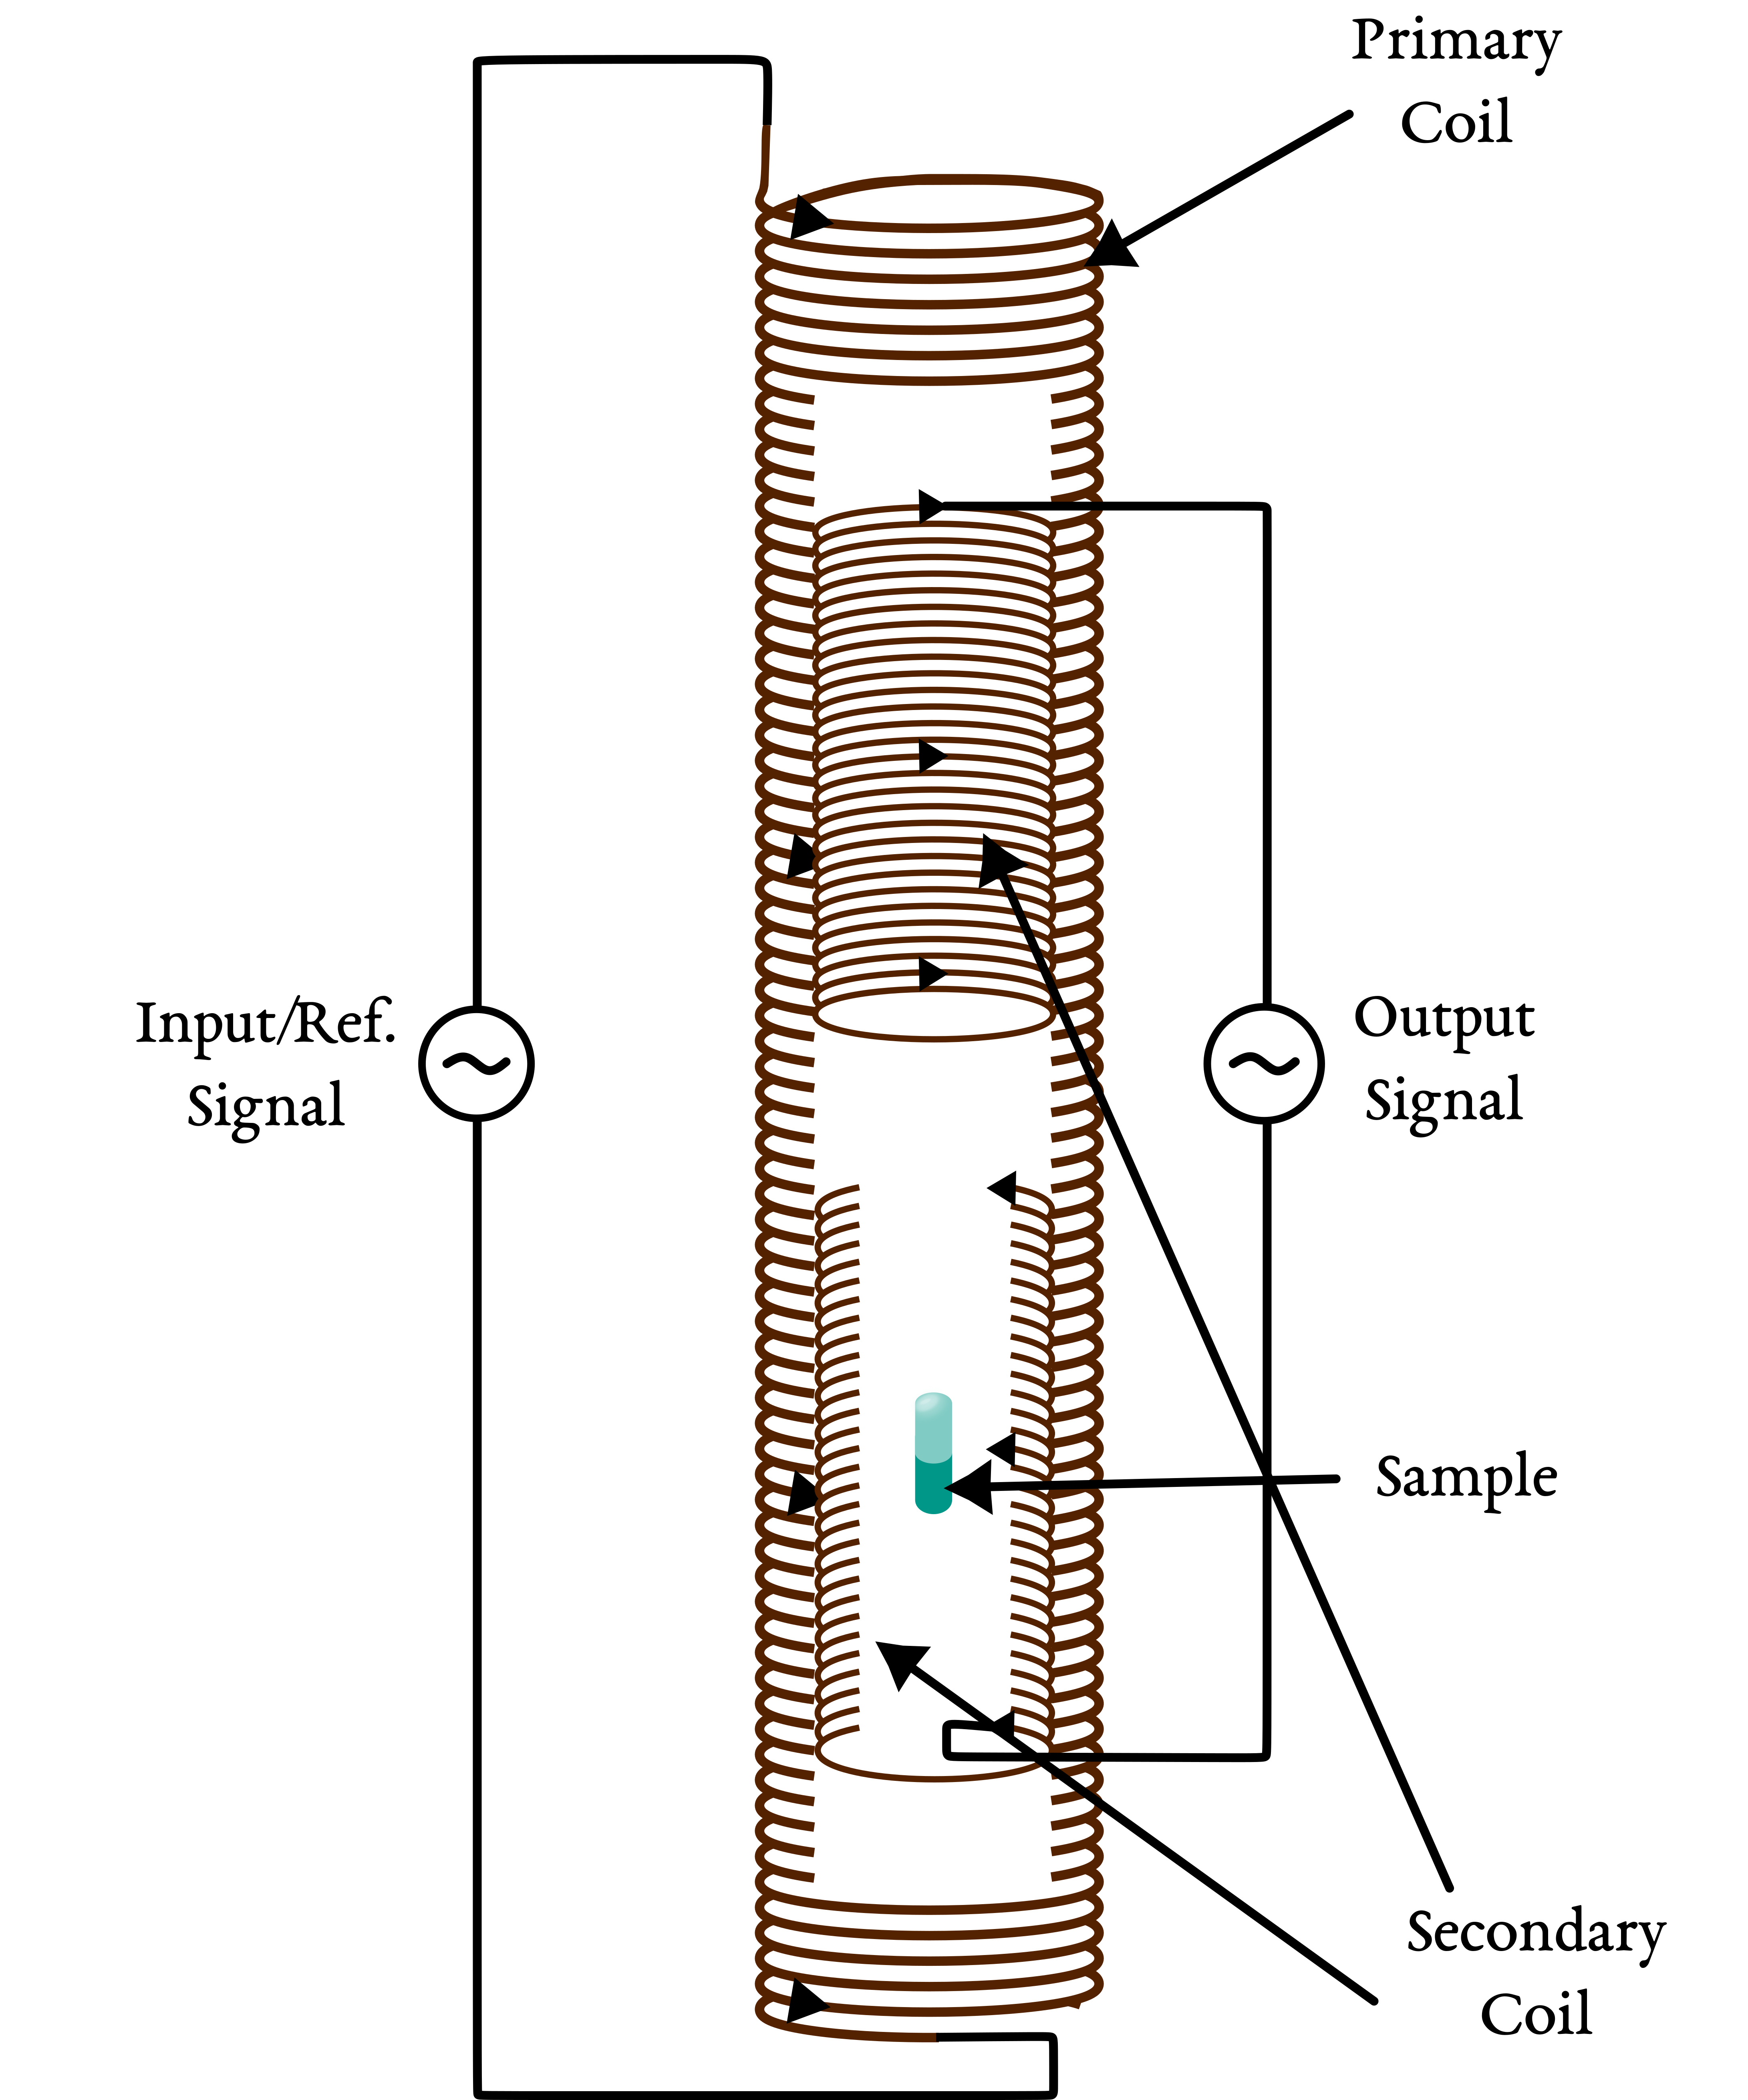
\includegraphics[width=0.8\textwidth]{coils.png}
  \label{assembly}
  \caption{This is main setup of experiment. you can see primary coil and tweo secondary coil winded opposite directions}
\end{figure*}

\subsection{Offset Settings}
At the initial stage, we have to offset null between two secondary coils voltage measurement. As a matter of facts we tried to take both our coils to be as symmetrical as possible but inherent human error is there. For this issue we took certain steps,

  
\vskip1cm
\begin{itemize}
\item Very crudely we take out or wind up our windings. This is to balance both secondary coils to almost perfection. This method is quite clumsy and pain staking. The offset still remains and we can’t go beyond the noise limit of the instrument.
\vskip1cm
\item Another thing we can do is that of using some external balancing circuit. Since we have very limited time we can’t go down this rabbit hole.
\end{itemize}
\vskip1cm
Finally we decided to ignore some offset and subtract it from data of samples. This way is not that effective but we don’t have other options.


\subsection{Calibration}
The giant task of our project was to calibrate our handmade instrument. This is also benign by noise of instruments and readings. We made a decision and did this the following way. As it turns out, Calibration can be done in two ways.\cite{cambr} 
\vskip1cm
\begin{itemize}
\item Theoretically, by mutual inductance cancellation. ((((ref 31)))
\vskip1cm
\item Experimentally, by taking some standard susceptibility values of some known and reliable sample.
\end{itemize}
\vskip1cm
There is still one catch, what we need is some $\chi_{int}$\cite{cambr}. What we are measuring is $\chi_{ext}$. What are these different susceptibilities? Well as it turns out the $\chi_{int}$ is what we expect from theoretically, 


\begin{equation*}
\chi_{int} = \frac{dM}{dH}
\end{equation*}
 And 
\begin{equation*}
\chi_{ext} = \frac{dM}{dH_a}
\end{equation*}
 
This two values are related by following identity (((ref camb paper))),

\begin{equation*}
\chi_{int} = \frac{\chi_{ext}}{1-D\chi_{ext}}
\end{equation*}

This value $\chi_{ext}$ is what we took proportional in the previous topic as LOCK IN’s output signal $V_{out}$. If we take the first equation then we can approximate the calibration constant to some extent, we took the second way that is experimental. We took some samples that can give out certain values of output. Before going there, we did the first method. Simplified setup for primary coil is shown in \ref{circuit}. Here we neglected the back inductance of the secondary coil.

\begin{figure}
  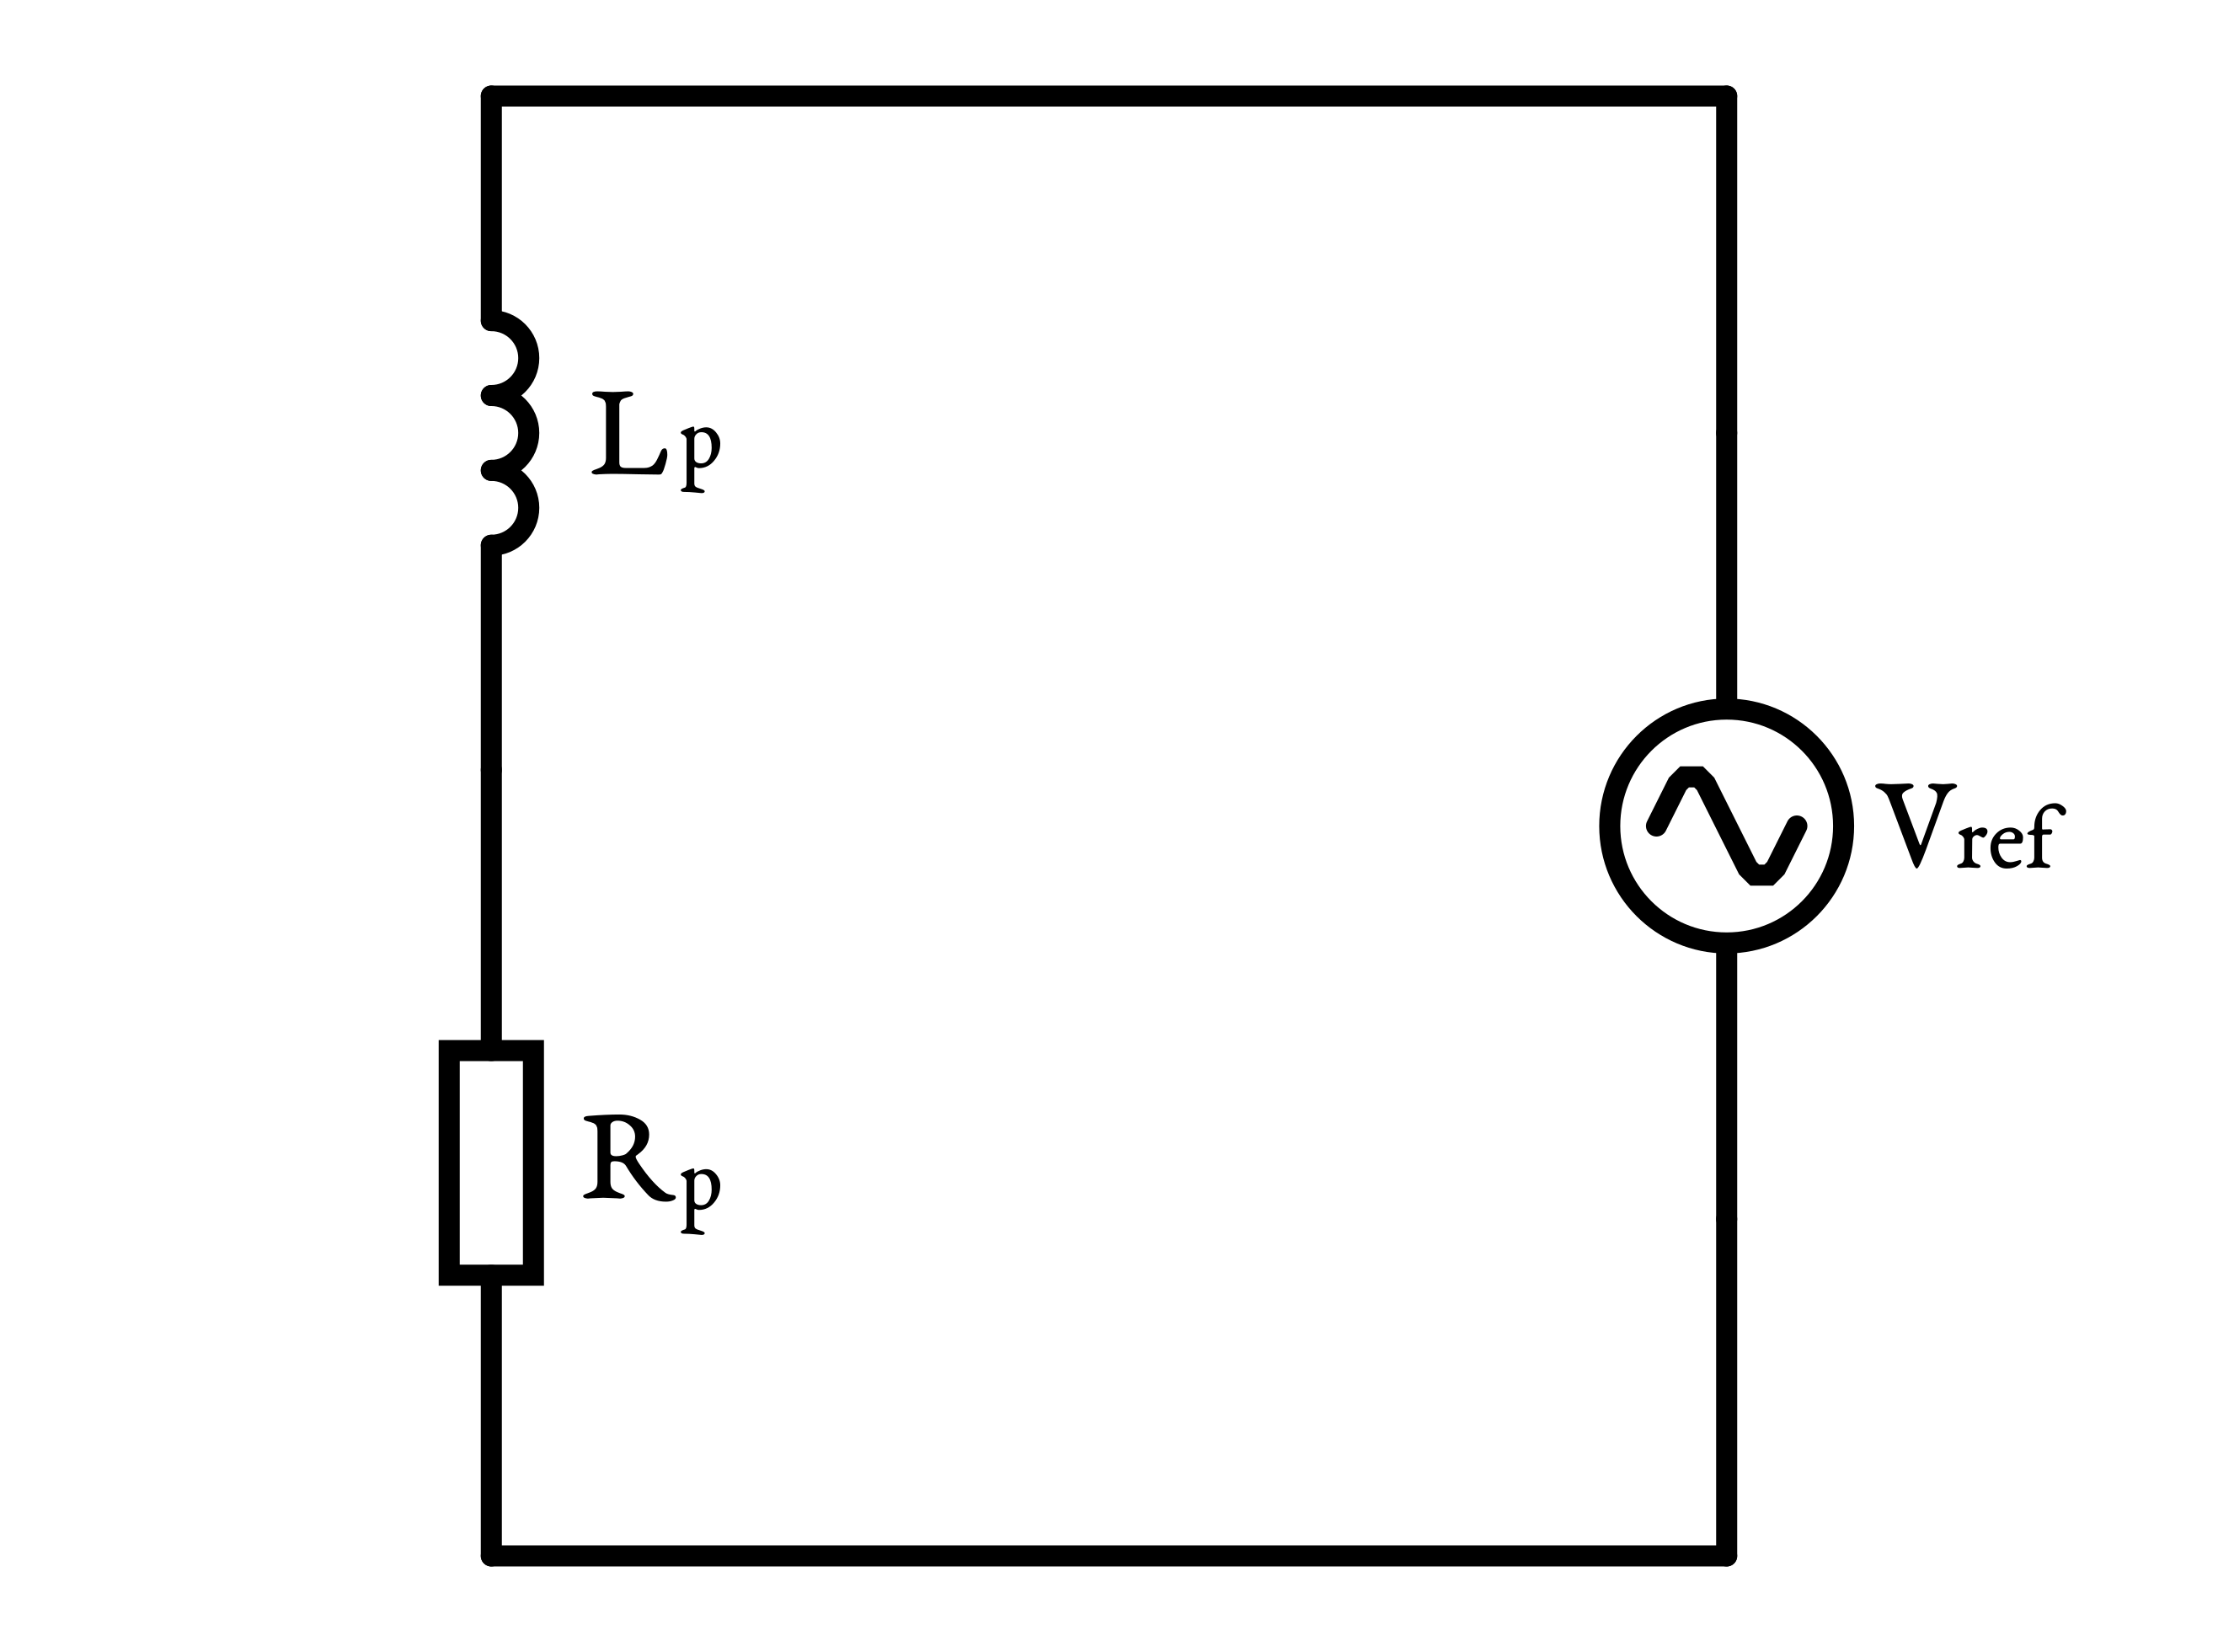
\includegraphics[width=1\linewidth]{circuit.png}
  \label{circuit}
  \caption{This is simpler circuit of coil assembly in our setup. we are neglecting effect of second coil}
\end{figure}

Simplified circuit makes following kind of differential equation,

\begin{equation}\label{diff}
  V_{in}-L\frac{dI}{dt}-IR=0
\end{equation}

Where, $V_{in}$ is nothing but $V_{ref}$ from the LOCK IN amplifier.  It is in the following form $V_{in} = V_0 e^{i(w_rt+\phi_r)}$, $w_r$ is applied frequency, $\phi_r$ is taken as zero from input. $I$ is currently in the primary, this parameter is very important and gives applied magnetic field strength $H_a$. $L$ and $R$ are both electrical parameters of the primary coil, respectively self-inductance and resistance. Solution of equation \ref{diff} gives current in primary at instance of time,

\begin{equation}
I_{real} = \frac{V_0\left[\frac{R}{L} cos(w_rt+\phi_r)+w_r sin(w_rt+\phi_r)\right]}{L(\frac{R^2}{L^2}+w_r^2)}+Ce^{-\frac{R}{L}t}  
\end{equation}

\begin{equation}
I_{imag}=\frac{\left[\frac{R}{L} sin(w_rt+\phi_r)-w_r cos(w_rt+\phi_r)\right]}{L(\frac{R^2}{L^2}+w_r^2)}
\end{equation}

If we take $\phi_r = 0$ and $V_0 = 1 V$ which signifies that total input phase and amplitude of reference voltage from LOCK IN amplifier is 0 deg and 1 V. Also, $C$ is an integral constant.
 

\begin{equation}
I_{real} = \frac{\frac{R}{L} cos(w_rt)+w_r sin(w_rt)}{L(\frac{R^2}{L^2}+w_r^2)}+Ce^{-\frac{R}{L}t}
\end{equation}

\begin{equation}
I_{imag}=\frac{\frac{R}{L} sin(w_rt)-w_r cos(w_rt)}{L(\frac{R^2}{L^2}+w_r^2)}
\end{equation}

 After taking condition that initial current is zero, 

\begin{equation}
C = \frac{-R}{L^2(\frac{R^2}{L^2}+w_r^2)}
\end{equation}

\begin{equation}
I_{real} = \frac{\frac{R}{L} cos(w_rt)+w_r sin(w_rt) -\frac{R}{L}e^{-\frac{R}{L}t}}{L(\frac{R^2}{L^2}+w_r^2)}
\end{equation}

From this current magnetic field strength inside primary coil and coupled by secondary coil is as following

\begin{equation*}
H_a(t) = c N I(t)
\end{equation*}

Which is measured in $A/m$, here $c$ is coupling constant for secondary coil. Since, the magnetic field inside the coil is not homogeneous, finding this parameter is very difficult, also if we find it then we get averaged out readings as whole coil. Magnetic field inside coil $B=\mu_0 H_a$. Also, flux inside secondary coil is as following, 

\begin{equation*}
\Phi = \mu_0 H_a n \pi a^2
\end{equation*}

Hare, $n$ and $a$ are geometrical parameters of the coil, $n$ is the number of turns of a single secondary coil and $a$ is the diameter of the secondary coil. We took the secondary coil in the centre of the primary coil as possible.
\begin{equation*}
\Phi = M I
\end{equation*}
\begin{equation*}
\frac{d\Phi}{dt} = M \frac{dI}{dt}
\end{equation*}

Here, $M$ is a mutual inductance parameter, which only depends on setup and sample placement. Final, voltage measurement from our secondary coil is only dependent is only LOCK IN readings ((ref camb paper)),

\begin{equation*}
V_{out} = \alpha H_a f V_{sample} \chi_{ext}
\end{equation*}

Here, $\alpha$ is calibration constant, which we have to determine. Theoretically, We know $H_a$, $V_{sample}$ (volume of sample: we took some small cylindrical capsule), $f$, $\chi_{ext}$ then we can find $\alpha$ directly. But knowing this parameter and their exact place in the instrument is very difficult. This is problematic. So, we turn to the second method and fix the orientations and parameters, put some sample and compare its reading calculated by their known magnetic susceptibility. 

For calibration purposes we took four samples and their readings of output voltages. These are 1. $Fe_2O_3$, 2. Nickel, 3. LSMO (Lanthanum strontium manganite), 4. $Gd_2O_3$. For characterization purposes $Fe_2O_3$ and $Gd_2O3$ are paramagnets where Nickel and LSMO are Ferromagnets. Problem we faced in our measurement is that our instrument’s sensitivity is very low and sample weight is very small. As a result paramagnetic substances have feeble signals which are not very reliable compared to ferromagnets like Nickel and LSMO. The data are shown in figures \ref{Rdata1}, \ref{Rdata2}, \ref{Rdata3} and \ref{Rdata4} where you can see why ferromagnets signal is reliable.

\begin{figure}[hbt!]
  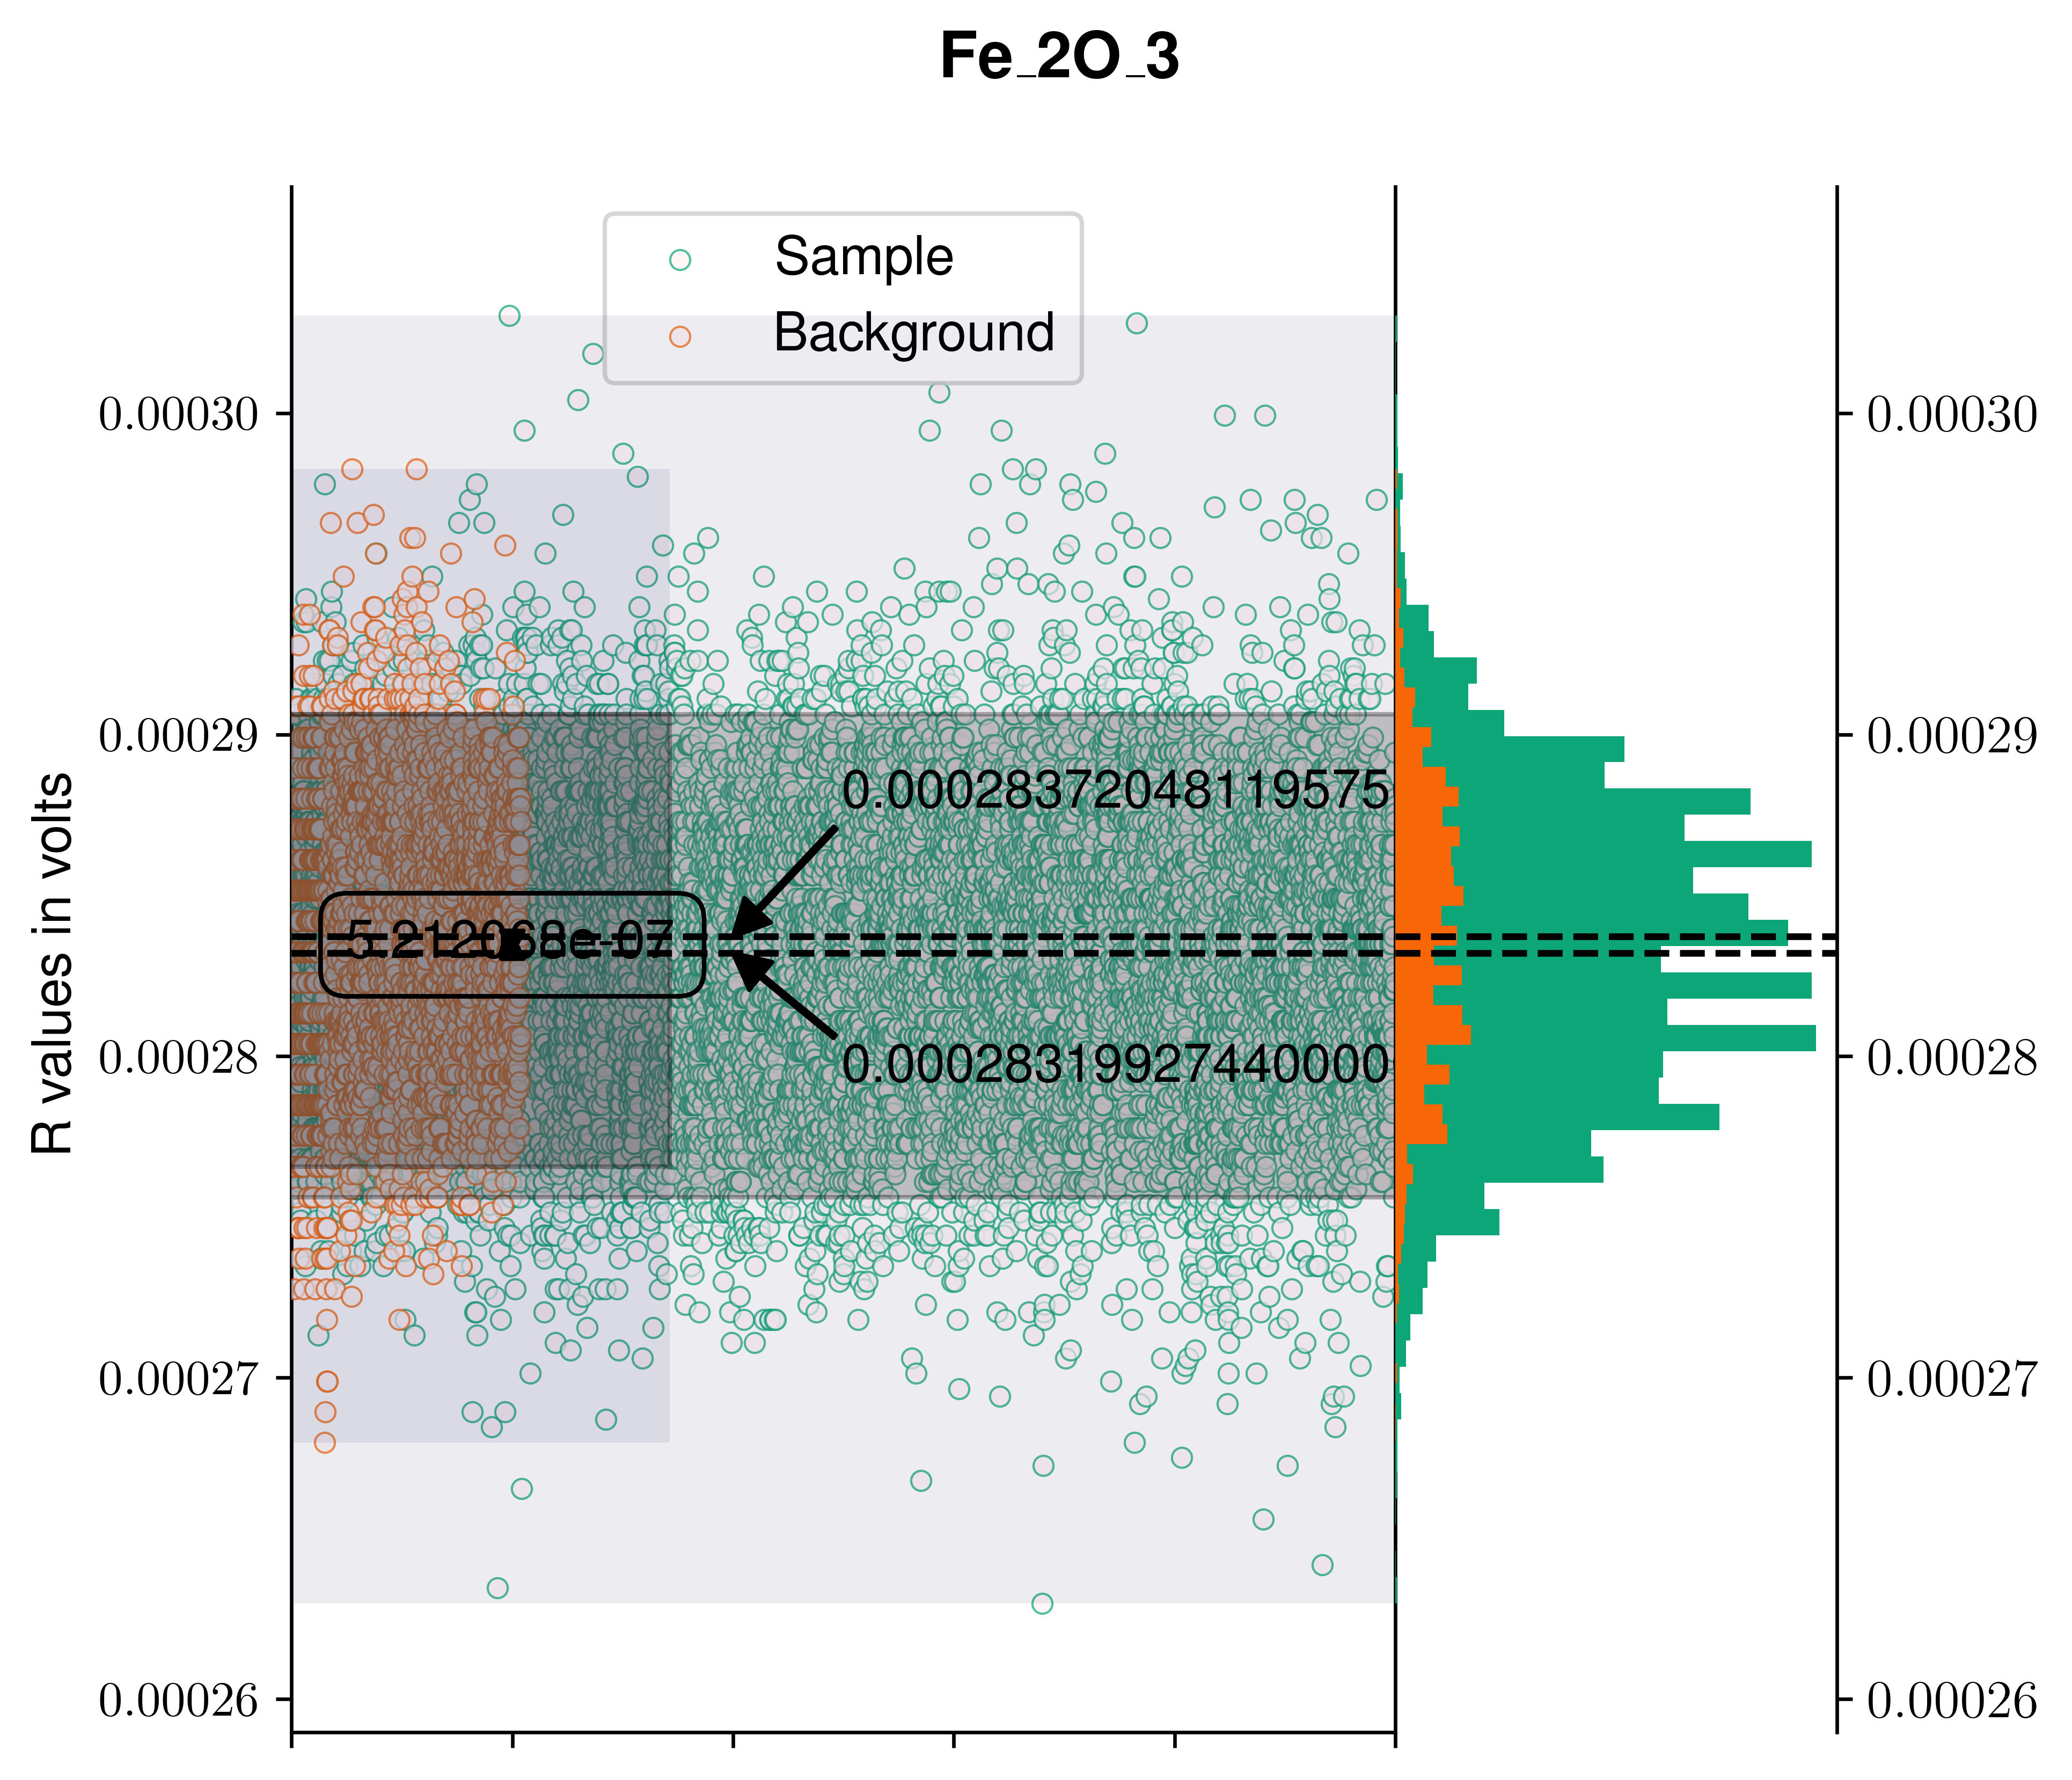
\includegraphics[width= \linewidth]{plots/fe2o3R.png}
  \label{Rdata1}
  \caption{Plot of absolute values of voltage $Fe_2O_3$ and it's Background. You can see difference is $5.212068 \times 10^{-7}$}
\end{figure}
\begin{figure}[hbt!]
  \includegraphics[width= \linewidth]{plots/gd2o3R.png}
  \label{Rdata2}
  \caption{Plot of absolute values of voltage $Gd_2O_3$ and it's Background. You can see difference is $3.543178 \times 10^{-7}$}
\end{figure}

Also values for Nickel and LSMO. You can see stark differences.

\begin{figure}[hbt!]
  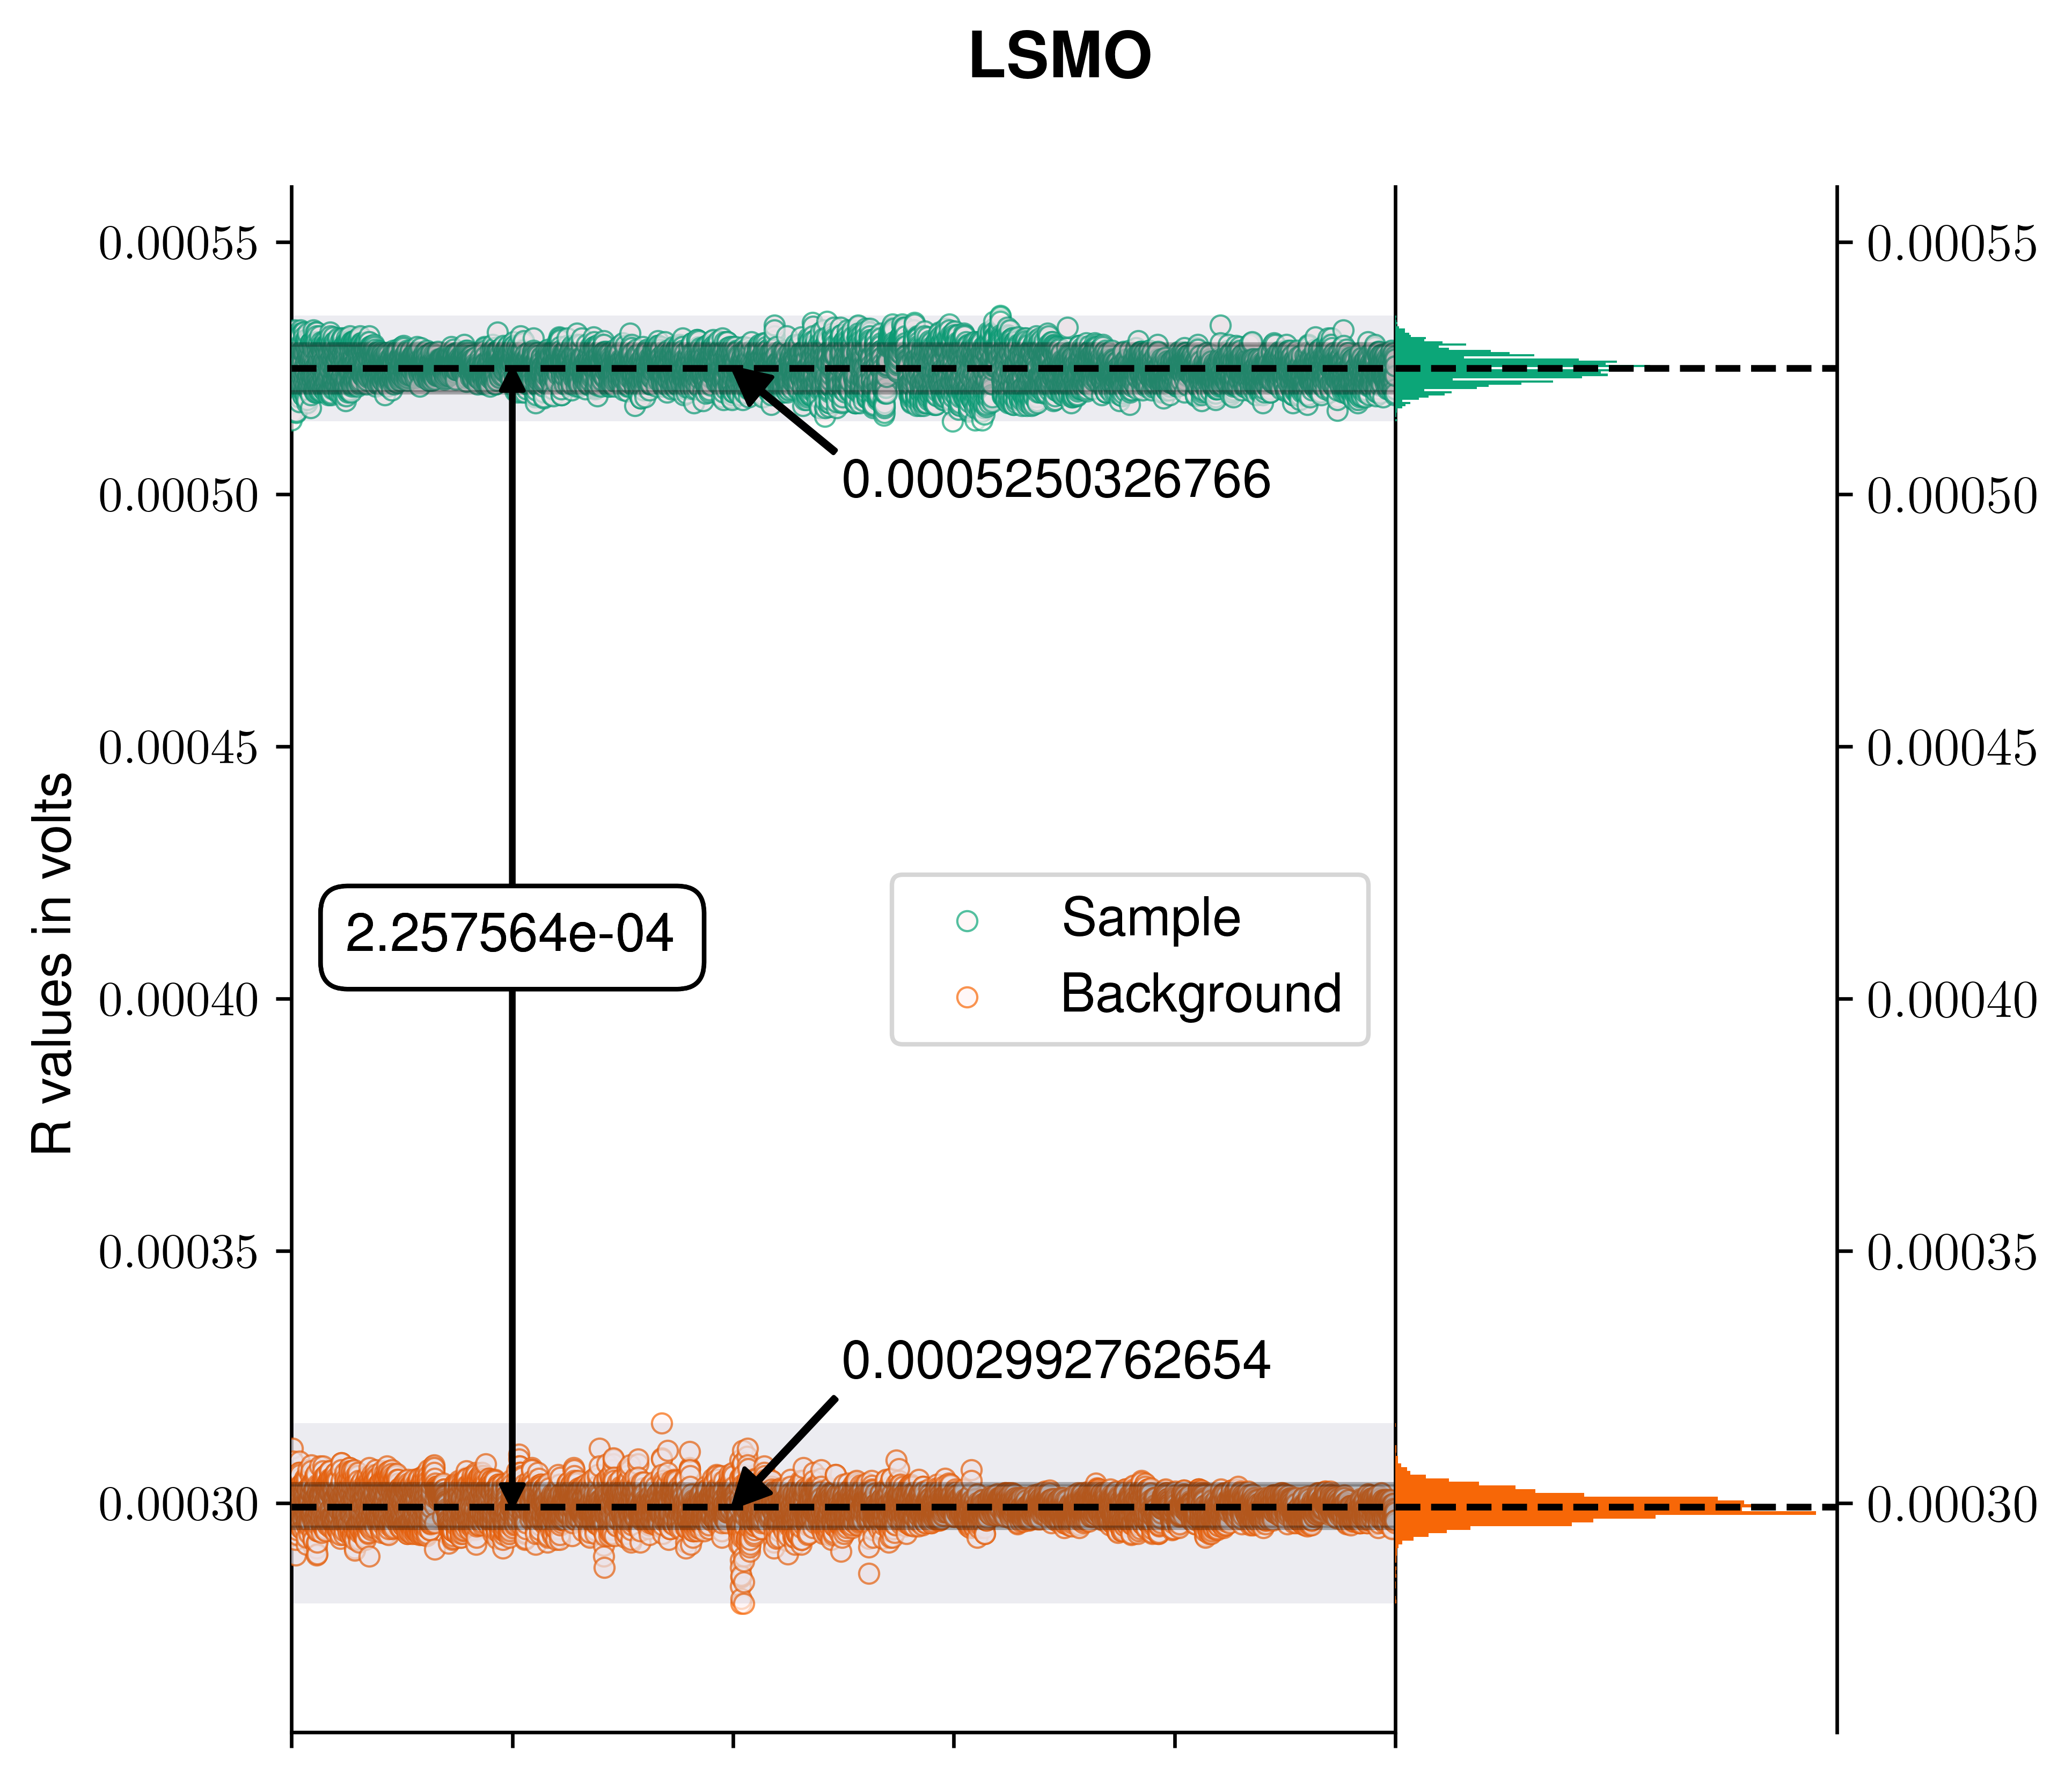
\includegraphics[width= \linewidth]{plots/LSMOR.png}
    \label{Rdata3}
  \caption{Plot of absolute values of voltage $LSMO$ and it's Background. You can see difference is $2.257564 \times 10^{-4}$}
\end{figure}
\begin{figure}[hbt!]
  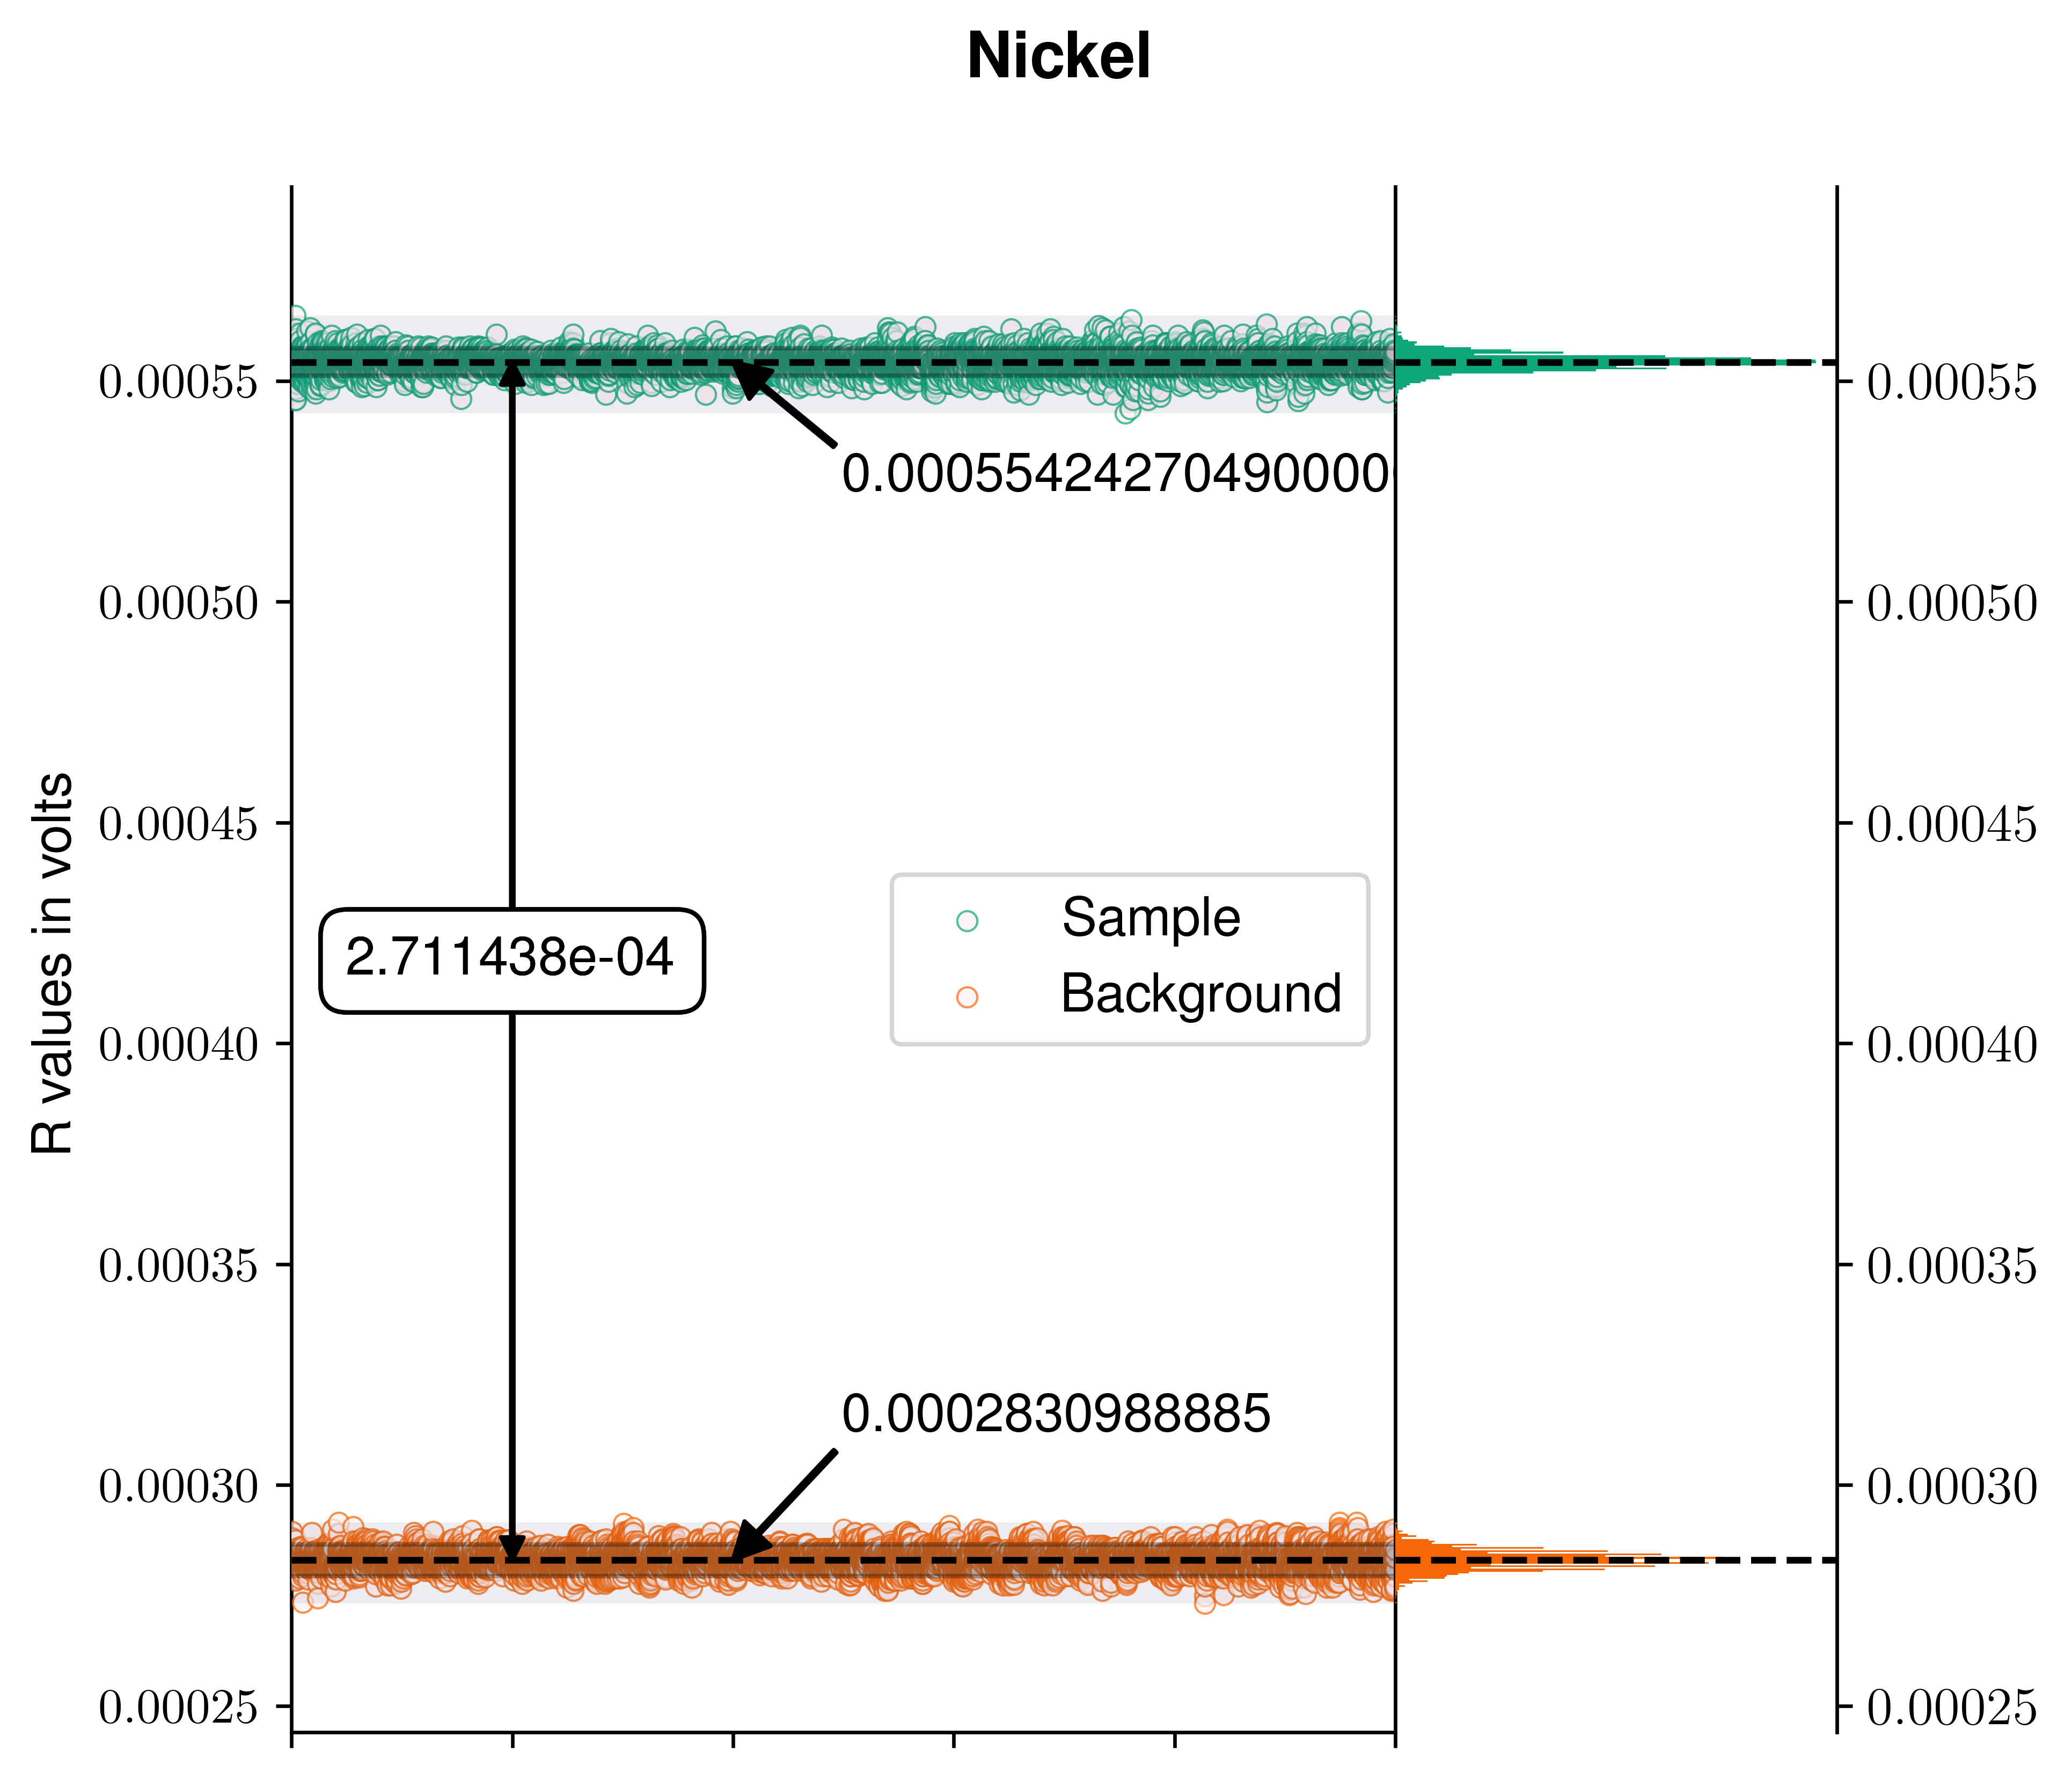
\includegraphics[width= \linewidth]{plots/nickelR.png}
    \label{Rdata4}
  \caption{Plot of absolute values of voltage Nickel and it's Background. You can see difference is $2.711438 \times 10^{-4}$}
\end{figure}

The values that we found in this data is that voltage differs relative to background(because we couldn’t make it zero). These values are shown in table \ref{Rreadings}.

\noindent\setlength\tabcolsep{4pt}%
\begin{tabularx}{\linewidth}{c|c}
  \hline
  \hline
  Samples & absolute voltage values in V \\
  \hline
  $Fe_2O_3$ & 30565445 \\
  $Gd_2O3$ & 20454545 \\
  Nickel & 457845454 \\
LSMO & 454544544 \\
\hline
\hline
\end{tabularx}
\label{Rreadings}
\captionof{table}{Absolute value reading after subtracting from background readings}
\vskip1cm

Now the big problem is that Susceptibility value of ferromagnets is too dependent on experiment parameters (magnetic field strength, frequency, temperature etc). Compared to it, paramagnets have almost constant value of magnetic susceptibility. As a consequence we could not find exact values of this material. We could only rely on approximate values of it. 

Also, we found $V_{in}$ and $V_{out}$ trends, which should directly give connection to magnetic susceptibility. This are that reading in figure \ref{voltage},

\begin{figure}[hbt!]
  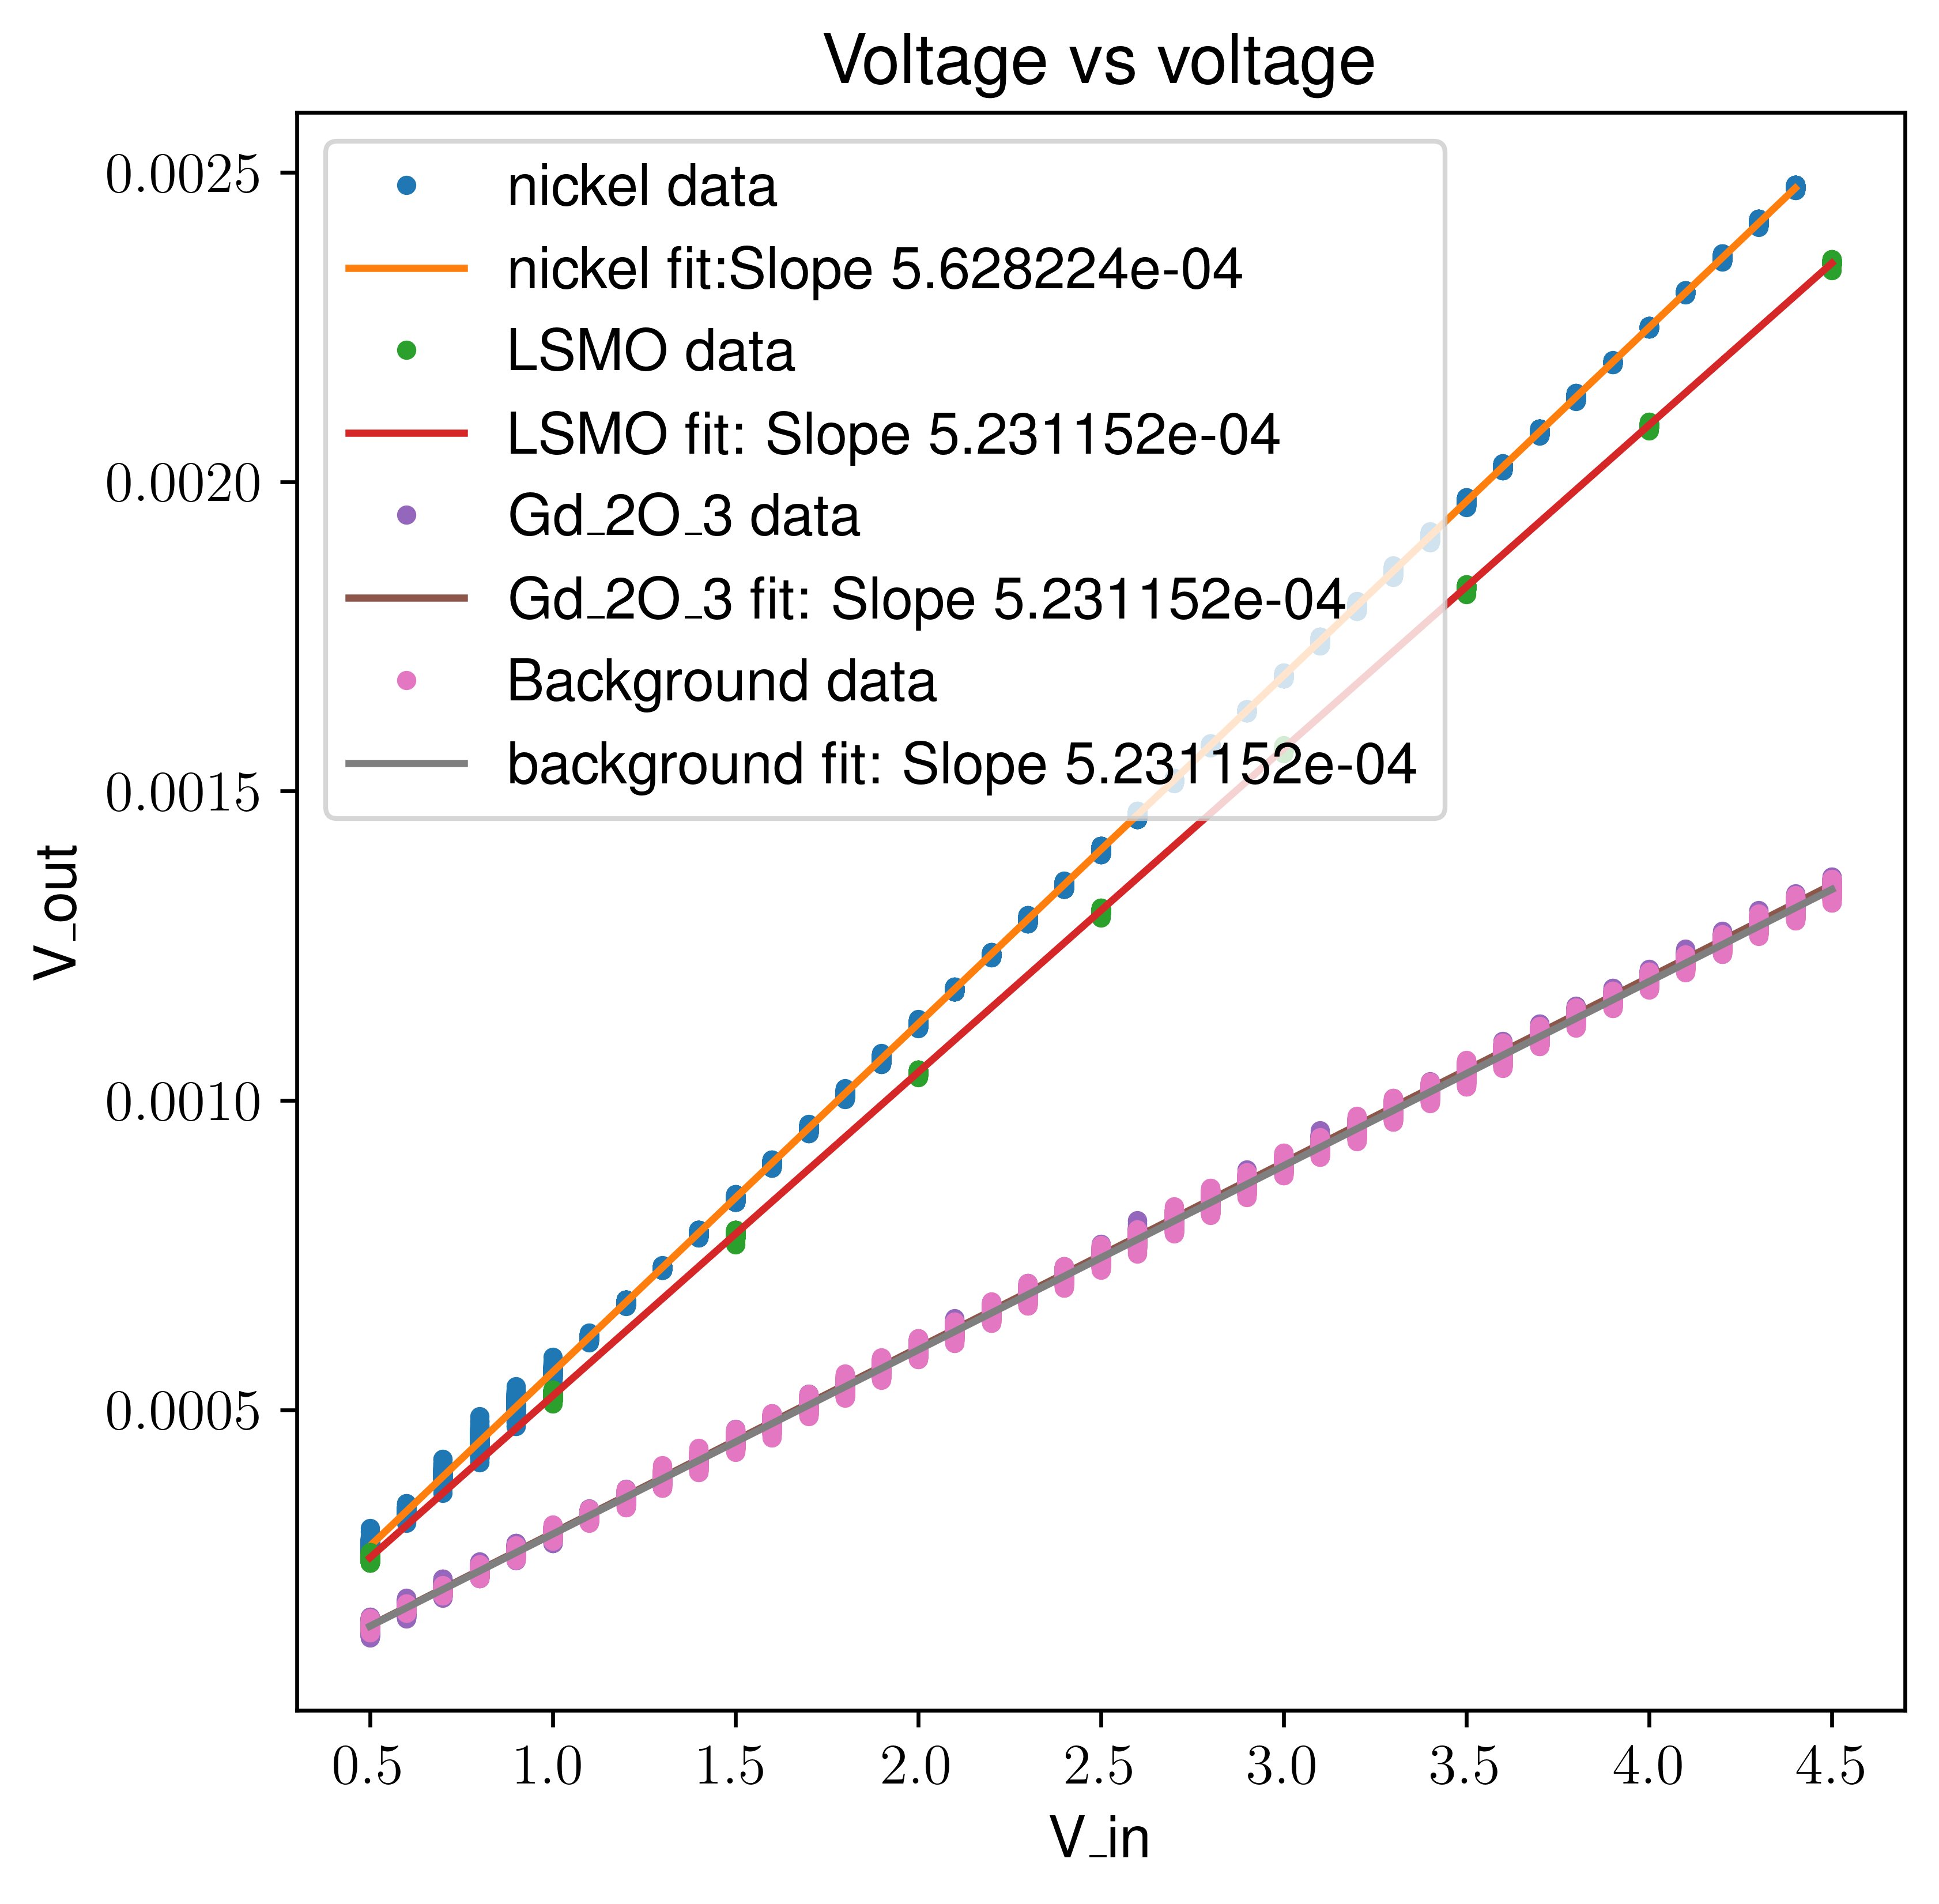
\includegraphics[width= \linewidth]{plots/voltage.png}
  \label{voltage}
  \caption{Different samples data for $V_{out}$ vs $V_{in}$}
\end{figure}

\noindent\setlength\tabcolsep{4pt}%
\begin{tabularx}{\linewidth}{c|c}
  \hline
  \hline
  Samples & Slope \\
  \hline
Nickel  & 5.62822393e-04 \\
LSMO  & 5.23115219e-04 \\
$Gd_2O_3$  & 2.99442997e-04 \\
Background  & 2.97732056e-04 \\
\hline
\hline
\end{tabularx}
\captionof{table}{Slopes readings of different samples $V_{out}$ vs $V_{in}$}
\label{Slopes}
\vskip1cm


This gives slopes of different samples and we can compare it to find ratios of different $\chi_{ext}$s. This relation should look like the following, $V_{out} \propto V_{in}$.
 
\begin{equation*}
V_{out} = \tau \chi_{ext} V_{in} 
\end{equation*}

Here, $\tau$ is some constant. From the data and above equation,  

\begin{equation*}
Slope \propto \chi_{ext}
\end{equation*}

\begin{equation*}
\frac{Slope^{(LSMO)}}{Slope^{(nickel)}} = \frac{\chi_{ext}^{(LSMO) sample}}{\chi_{ext}^{(nickel) sample}}
\end{equation*}

Here, $\chi_{ext}^{sample}= \frac{W \chi_{ext}}{W_a}$, where $W$ and $W_a$ are weight and atomic weight.

\begin{equation*}
\frac{5.23115219e-04}{5.62822393e-04} = \frac{(0.2906 g)\chi_{ext}^{(LSMO) \times (58.693)}}{(0.1942 g)\chi_{ext}^{(nickel)} \times (226.45)}
\end{equation*}

\begin{equation*}
1.075905 = \frac{\chi_{ext}^{(LSMO)}\times 17.0562}{\chi_{ext}^{(nickel)} \times 43.9766}
\end{equation*}

\begin{equation*}
2.77404 \times \chi_{ext}^{nickel} = \chi_{ext}^{(LSMO)}
\end{equation*}

For nickel we took magnetic susceptibility about $\chi_{int}^{(nickel)}=0.004423 m^3/mol$.

If we put these values in equation ((reference)). This gave us a value of $\alpha = 11.82249$. This value is relatively high, which signifies sensitivity of our instrument. Compare it to values of some other commercial and also from other experiments, we have very $\frac{1}{\alpha}=0.08485 Am^2V^{-1}s^{-1}$ is low compared to commercials around $2.1546Am^2V^{-1}s^{-1}$ and from one experiment $11.24 Am^2V^{-1}s^{-1}$\cite{cambr}.


\subsection{Noise}
Noise factor in our instrument is very high. For Example the $R$ values which are absolute values of voltage ($\sqrt{X^2+Y^2}$) have relatively less noise compared to phase measurement. These noise values can’t be ignored since our measurements will have a relatively low number of measurements and the signal will be very feeble.

LOCK IN in our setup is a very low noise instrument. This is a good thing to start with but as we built our instrument this factor is not very important. Instrument noise in our setup is very high for coils and other things. We take certain steps to reduce it, for example we made Faraday's cage like structure from aluminium foil to reduce external interference. 

After doing all this we have very significant noise in our setup. Take a comparison between $R$ values of samples and phase measurement of the system. Compare this figures \ref{Tdata1}, \ref{Tdata2}, \ref{Tdata3} and  \ref{Tdata4} to the $R$ measurement given on this figure \ref{Rdata1}, \ref{Rdata2}, \ref{Rdata3}, \ref{Rdata4}.

begin{figure}[hbt!]
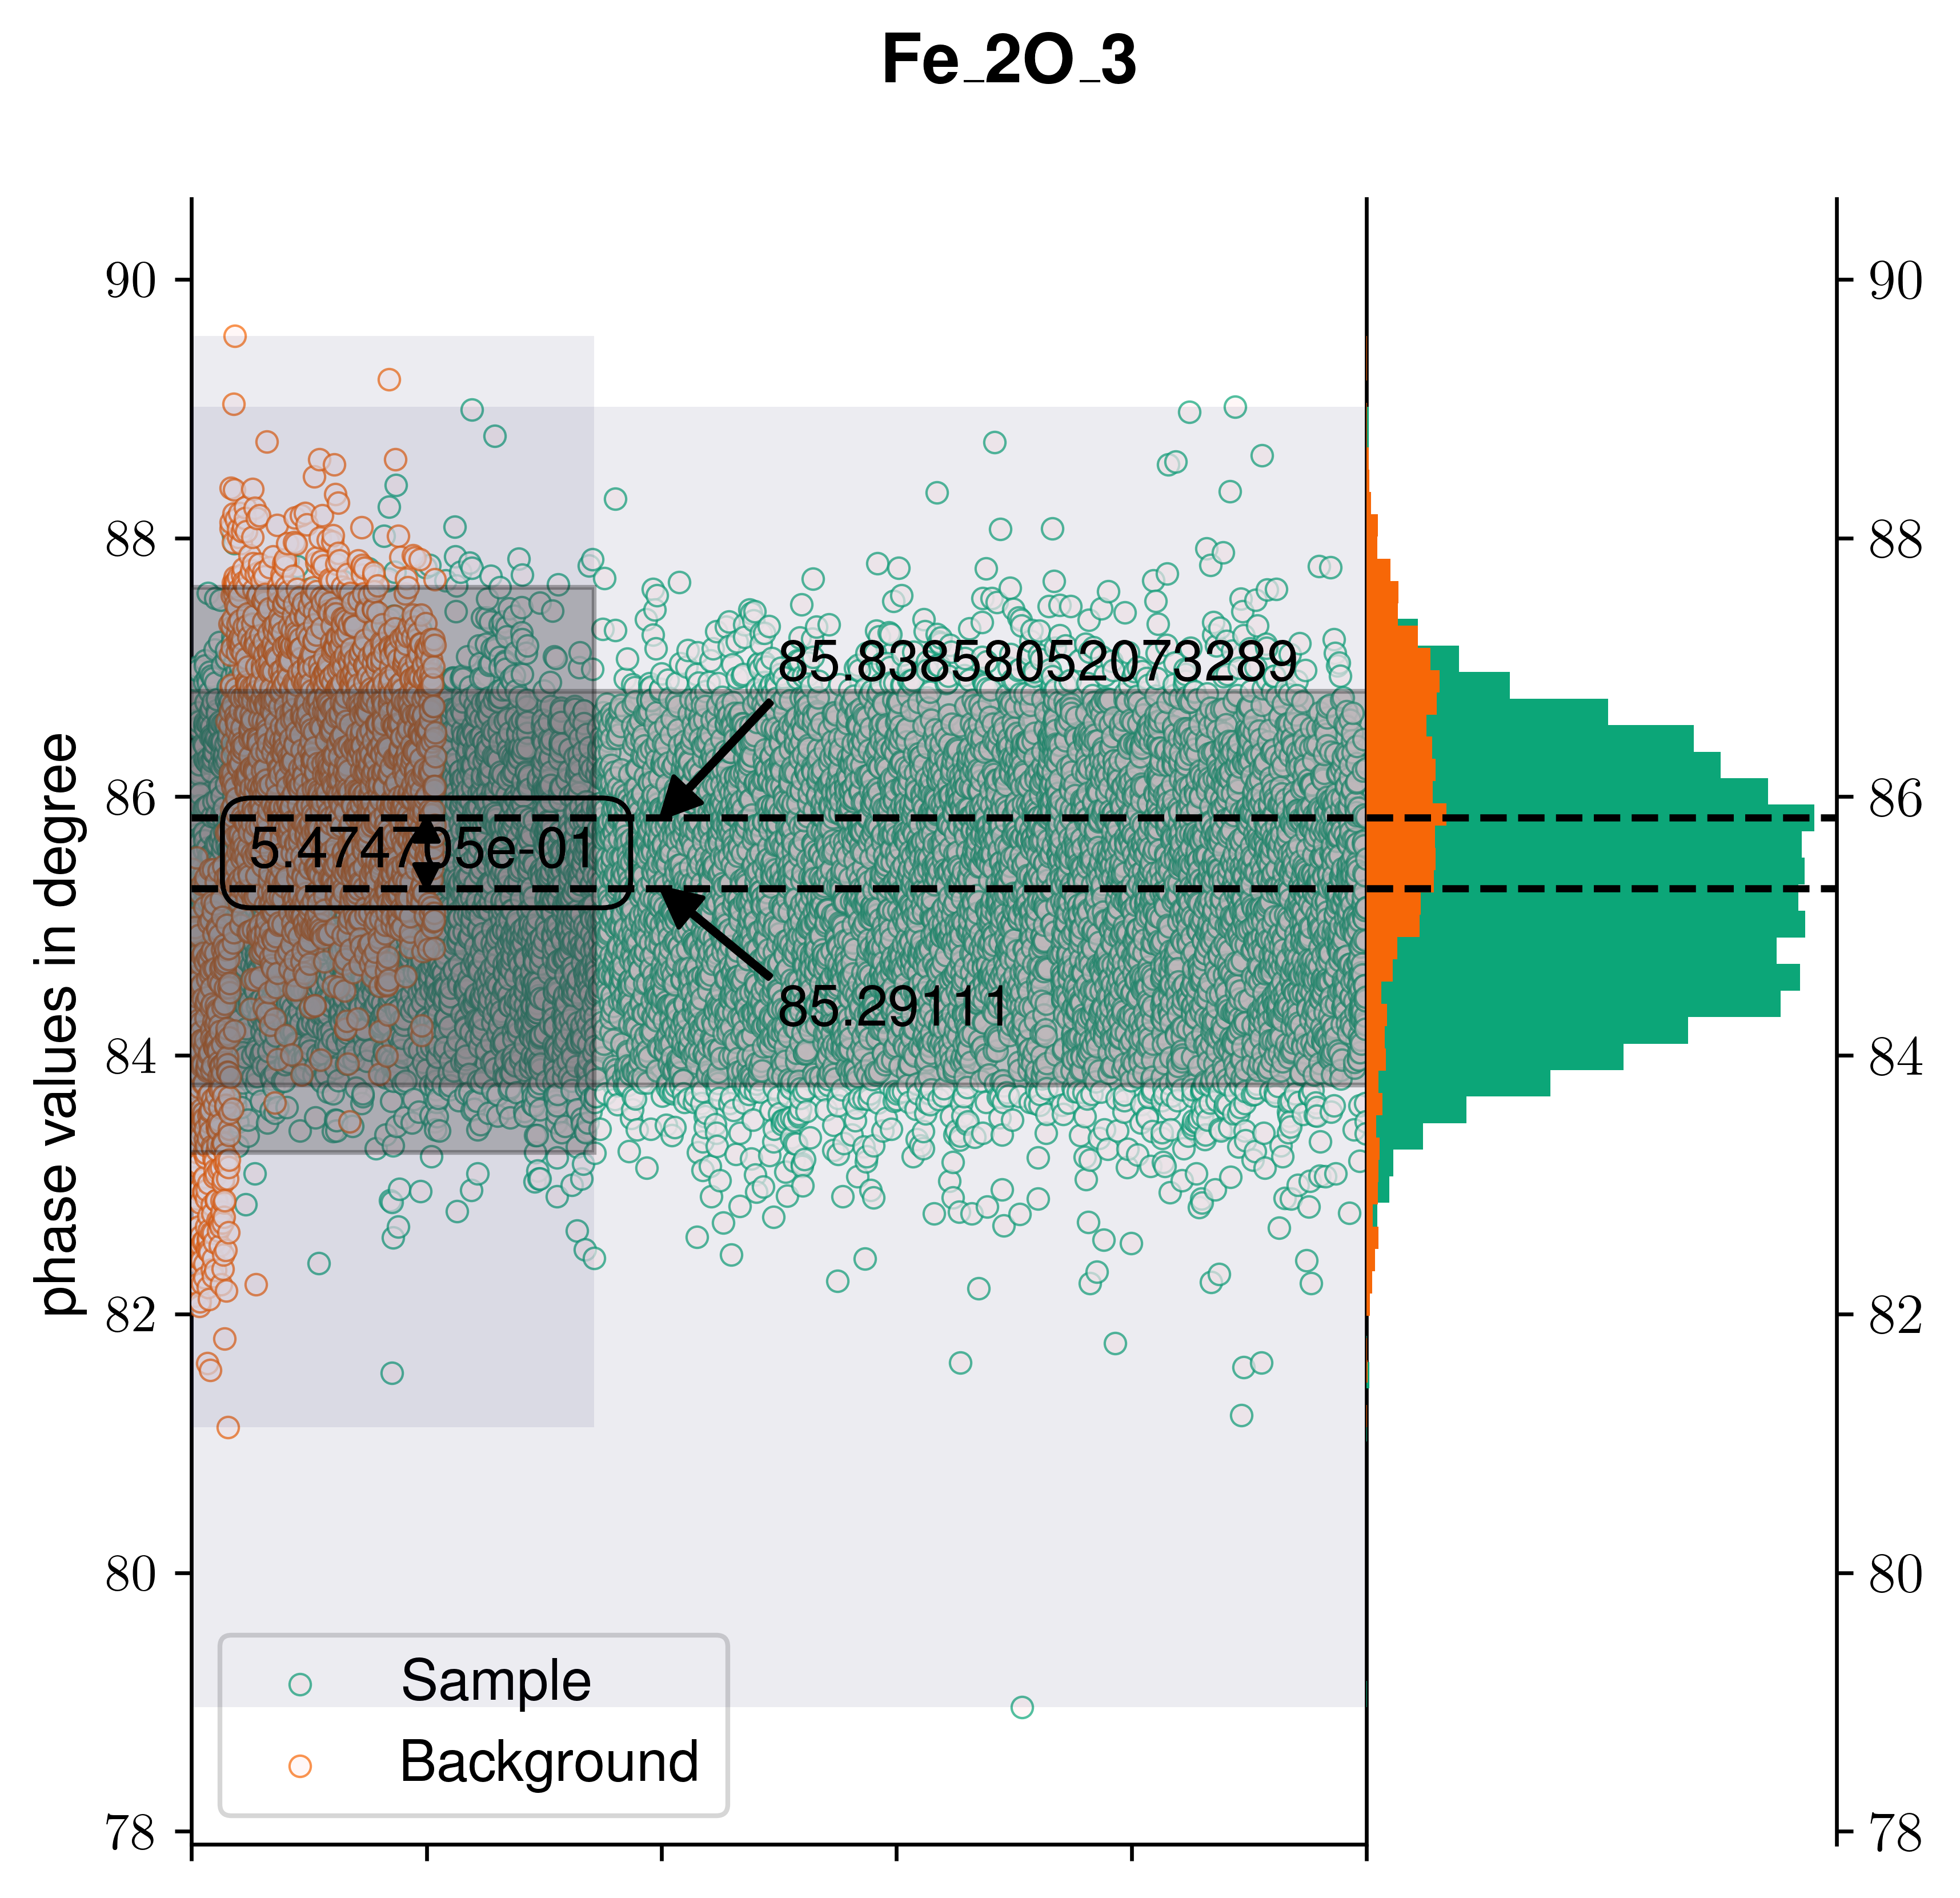
\includegraphics[width= \linewidth]{plots/fe2o3T.png}
\label{Tdata1}
\caption{Plot of phase values in degree $Fe_2O_3$ and it's Background}
\end{figure}
\begin{figure}[hbt!]
  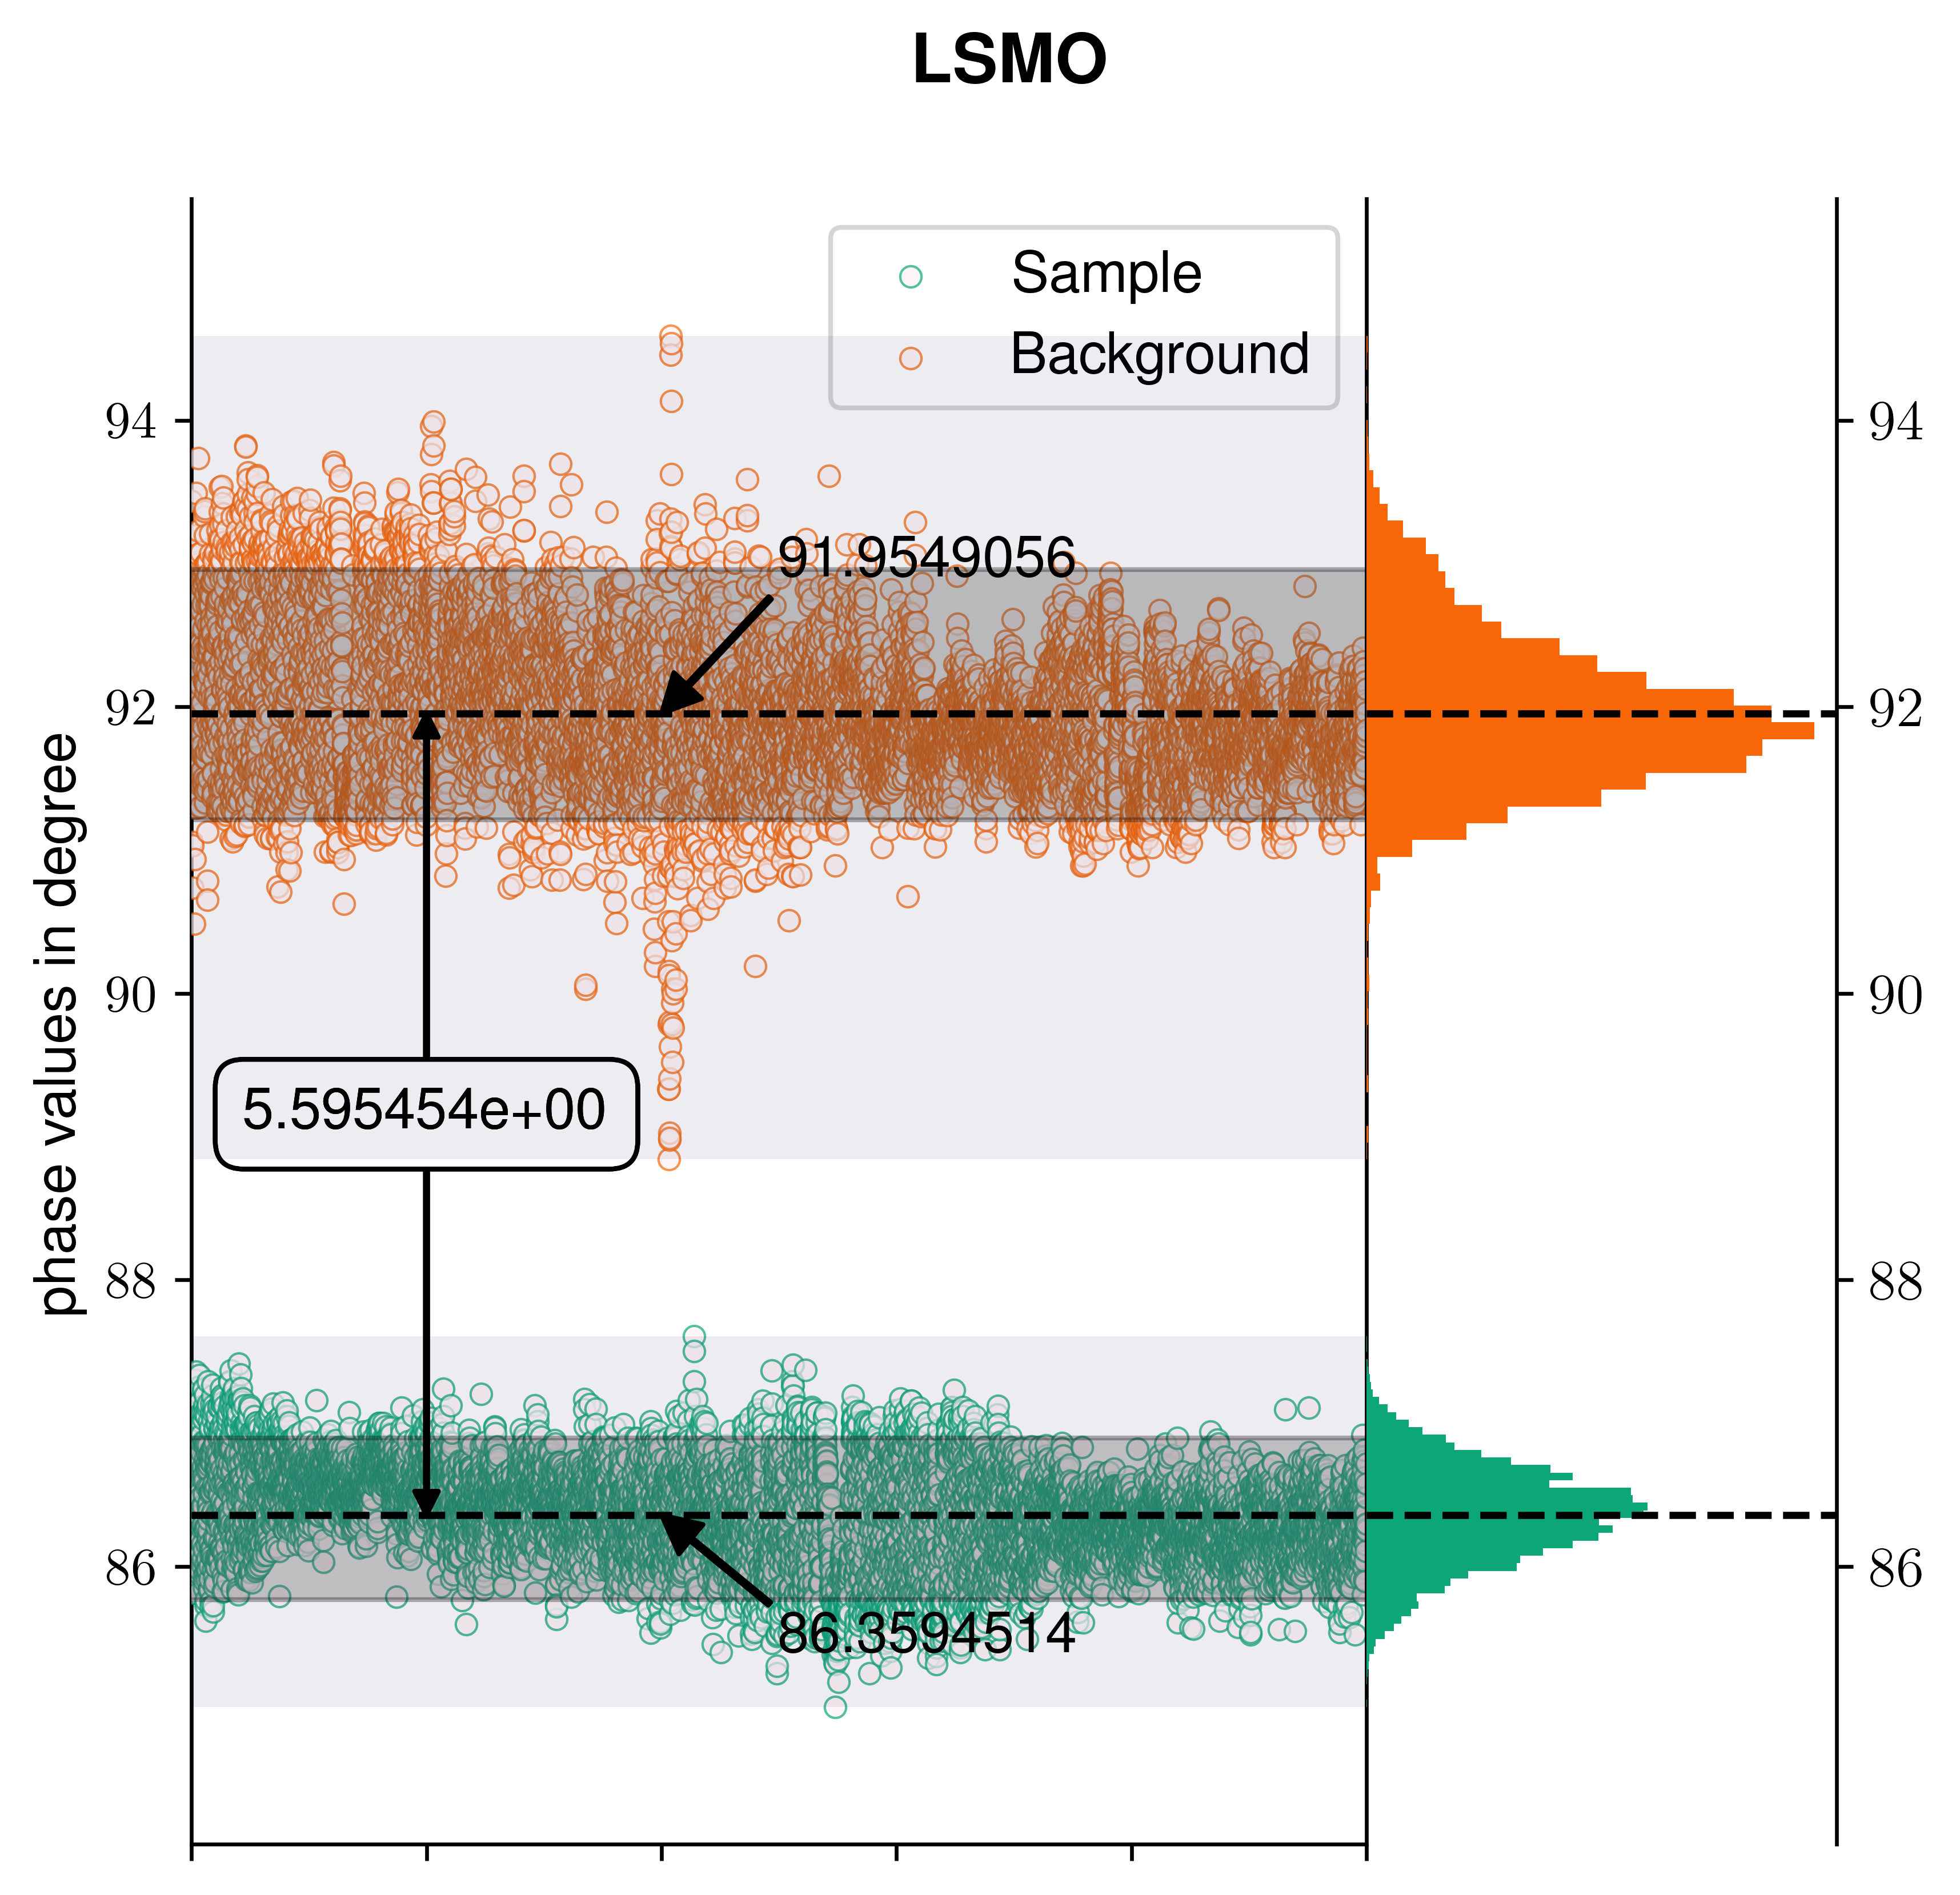
\includegraphics[width= \linewidth]{plots/LSMOT.png}
  \label{Tdata2}
  \caption{Plot of phase values in degree $Gd_2O_3$ and it's Background}
\end{figure}
\begin{figure}[hbt!]
  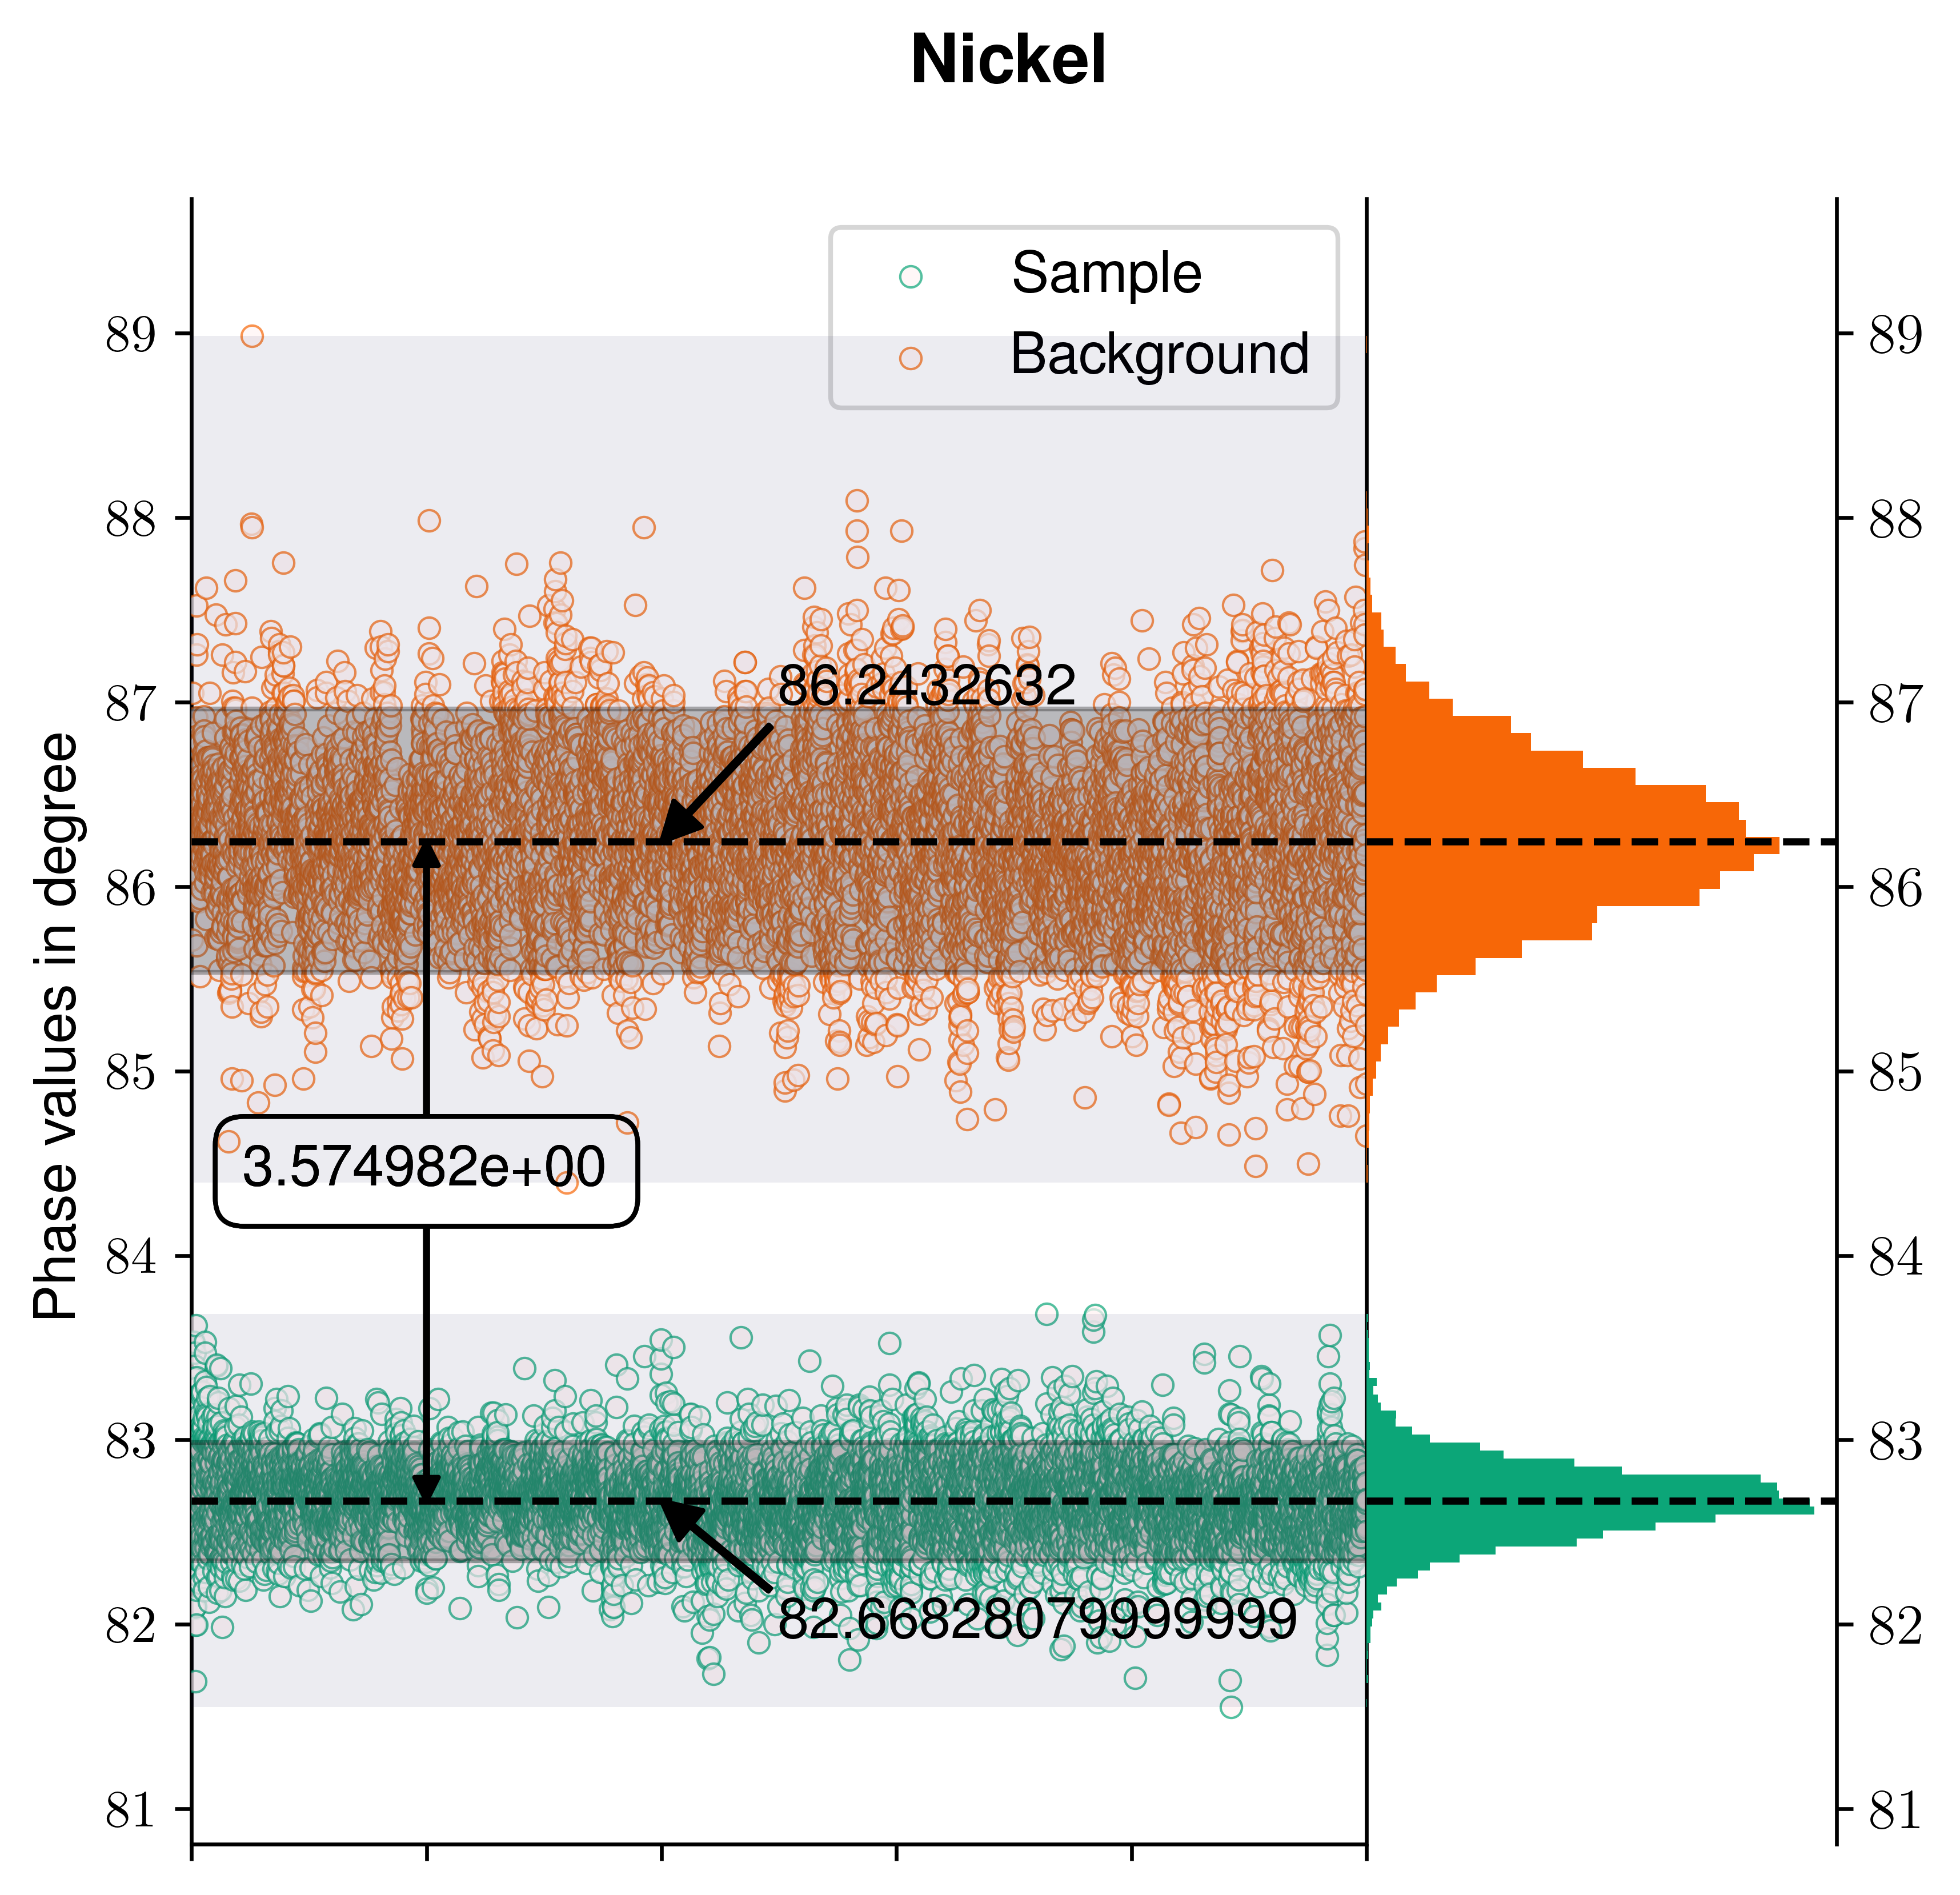
\includegraphics[width= \linewidth]{plots/nickelT.png}
  \label{Tdata3}
  \caption{Plot of phase values in degree $LSMO$ and it's Background}
\end{figure}
\begin{figure}[hbt!]
  \includegraphics[width= \linewidth]{plots/gd2o3T.png}
  \label{Tdata4}
  \caption{Plot of phase values in degree Nickel and it's Background}
\end{figure}
